\documentclass[11pt]{article}


% TODO: use polyflossia
\usepackage[english, spanish]{babel}

% font specification
\usepackage{fontspec}
% \setmainfont{TeX Gyre Pagella}
% \setmainfont[Mapping=tex-text]{TeX Gyre Pagella}
% \setmainfont[Ligatures=TeX]{TeX Gyre Pagella}

\setmainfont[Mapping=tex-text]{LinLibertineO}
\newfontfamily\ipa{LinLibertineO}

% \setsansfont[Scale=MatchLowercase]{Latin Modern Sans}
% \setsansfont[Scale=MatchLowercase]{Linux Biolinum O}
\setsansfont[Scale=MatchLowercase]{Carlito}

% consolas no es free pero tiene bold, inconsolata es al vesre
% \setmonofont[Scale=MatchLowercase]{Inconsolata}
% \setmonofont[Scale=MatchLowercase]{Consolas}
\setmonofont[Scale=MatchLowercase]{DejaVu Sans Mono}

% page sizes and margins
\usepackage{geometry}
\geometry{paper=a4paper, left=2.75cm, right=2.75cm, bottom=2.5cm, foot=2cm, top=3.5cm}
\setlength{\headheight}{14pt}

% hyperlinks in pdfs
\usepackage{hyperref}
\hypersetup{pdftitle=, pdfauthor=,pdfborder={0 0 0}, colorlinks=false, linkcolor=black, citecolor=black, filecolor=black}
\hypersetup{pdftitle={Resolución de la ecuación de transporte mediante el método de las características en el código neutrónico milonga}, pdfauthor={Ramiro Vignolo}}

% headers & footers
\usepackage{fancyhdr}
\makeatletter
\fancyhead[L]{}
\fancyhead[C]{}
\fancyhead[R]{\thepage/\pageref{lastpage}}
\fancyfoot[L]{}
\fancyfoot[C]{\tiny{\texttt{Asociación Argentina de Tecnología Nuclear}}}
% \fancyfoot[R]{\thepage}
\fancyfoot[R]{}
\makeatother
\renewcommand{\headrulewidth}{0.4pt}
% \renewcommand{\footrulewidth}{0.4pt}
\pagestyle{fancy}

% biblatex
\usepackage{csquotes}     % this package is needed for \blx@bibinit below (sic)
\usepackage[backend=biber,sorting=none]{biblatex}    
\addbibresource{bibliografia/bibliografia.bib}
\addbibresource{bibliografia/congresos.bib}
\addbibresource{bibliografia/informes.bib}
\addbibresource{bibliografia/internacionales.bib}
\addbibresource{bibliografia/monografias.bib}
\addbibresource{bibliografia/nacionales.bib}
% initialize macros so \bibstring can be used to show some fields (needs csquotes)
\makeatletter
\blx@bibinit
\makeatother

% Font style for figures' and tables' captions
\usepackage[small,bf,up]{caption}
\renewcommand{\captionfont}{\scriptsize\sf}

% things
\usepackage{lastpage}
\usepackage{graphicx}
\usepackage{amsmath}
\usepackage{amssymb}
\usepackage{rotating}
\usepackage{tabularx}
\usepackage[table]{xcolor}
\usepackage{eso-pic}
\usepackage{subfig}
\usepackage{listings}
\usepackage{xltxtra}
\usepackage{siunitx}

% remember to run
%  $ ./syntax-tex.sh > wasora-keywords
\lstdefinelanguage{wasora}{
morekeywords={
      MILONGA_PROBLEM,
      GROUPS,
      FORMULATION,
      TRACK,
      TRACK_MESH,
      N_AZIM_ANGLES,
      TRACK_SPACING,
      TRACK_DENS,
      TINY_STEP,
      DO_NOT_CHECK_VOLUMES,
      POLAR_QUADRATURE,
      N_POLAR_ANGLES,
      TYPE,
      LOAD_PLUGIN,
      DEFAULT_ARGUMENT_VALUE,
      INCLUDE,
      FROM,
      TO,
      ABORT,
      IMPLICIT,
      DO_NOT_EVALUATE_AT_PARSE_TIME,
      TIME_PATH,
      INITIAL_CONDITIONS_MODE,
      LOAD_ROUTINE,
      VAR,
      CONST,
      ALIAS,
      IS,
      AS,
      VECTOR,
      SIZE,
      DATA,
      FUNCTION_DATA,
      MATRIX,
      ROWS,
      COLS,
      FUNCTION,
      FILE_PATH,
      ROUTINE,
      MESH,
      NODES,
      CELLS,
      VECTOR_DATA,
      VECTORS,
      COLUMNS,
      INTERPOLATION_THRESHOLD,
      INTERPOLATION,
      FILE,
      OUTPUT_FILE,
      INPUT_FILE,
      MODE,
      INPUT,
      OUTPUT,
      OPEN,
      DO_NOT_OPEN,
      CLOSE,
      IF,
      ELSE,
      ENDIF,
      SEMAPHORE,
      SEM,
      READ,
      WRITE,
      SHM,
      SHM_OBJECT,
      ASCII_FILE_PATH,
      BINARY_FILE_PATH,
      ASCII_FILE,
      BINARY_FILE,
      IGNORE_NULL,
      PRINT,
      NONEWLINE,
      SEP,
      SEPARATOR,
      NOSEP,
      HEADER,
      STRING,
      TEXT,
      PRINT_FUNCTION,
      MIN,
      MAX,
      STEP,
      NSTEPS,
      FORMAT,
      PRINT_VECTOR,
      VERTICAL,
      HORIZONTAL,
      ELEMS_PER_LINE,
      SOLVE,
      UNKNOWNS,
      RESIDUALS,
      GUESS,
      METHOD,
      EPSABS,
      EPSREL,
      MAX_ITER,
      VERBOSE,
      M4,
      INPUT_FILE_PATH,
      OUTPUT_FILE_PATH,
      MACRO,
      SHELL,
      CALL,
      HISTORY,
      PARAMETRIC,
      TYPE,
      OUTER_STEPS,
      MAX_DAUGHTERS,
      OFFSET,
      ADIABATIC,
      FIT,
      VIA,
      GRADIENT,
      RANGE_MIN,
      RANGE_MAX,
      DELTAEPSREL,
      DELTAEPSABS,
      DO_NOT_RERUN,
      NORERUN,
      RERUN,
      MINIMIZE,
      OPTIMIZE,
      SIMAN_EFUNC,
      ALGORITHM,
      PHASE_SPACE,
      DIFFERENTIAL,
      NAME,
      STRUCTURED,
      DIMENSIONS,
      SCALE_FACTOR,
      OFFSET_X,
      OFFSET_Y,
      OFFSET_Z,
      DEGREES,
      NCELLS_X,
      NCELLS_Y,
      NCELLS_Z,
      LENGTH_X,
      LENGTH_Y,
      LENGTH_Z,
      DELTA_X,
      DELTA_Y,
      DELTA_Z,
      MESH_POST,
      NOMESH,
      NO_MESH,
      CELL_CENTERED,
      NODE_CENTERED,
      MESH_FILL_VECTOR,
      EXPRESSION,
      EXPR,
      PHYSICAL_ENTITY,
      ID,
      MATERIAL,
      BOUNDARY,
      BC,
      INCREMENTAL,
      PHYSICAL_PROPERTY,
      NONE,
      ALLOWED,
      AS_PROVIDED,
      FROM_VARIABLES,
      FROM_DERIVATIVES,
      WAIT,
      POST,
      SKIP_STEP,
      SKIP_STATIC_STEP,
      SKIP_TIME,
      SKIP_HEADER_STEP,
      MAX_ITER,
      TOL,
      GRADTOL,
},
morekeywords={[2]
},
morekeywords={[3]
      cells,
      cells_0,
      done,
      done_0,
      done_outer,
      done_outer_0,
      done_static,
      done_static_0,
      done_transient,
      done_transient_0,
      dont_quit,
      dont_quit_0,
      dont_report,
      dont_report_0,
      dt,
      dt_0,
      elements,
      elements_0,
      end_time,
      end_time_0,
      eps,
      eps_0,
      i,
      i_0,
      infinite,
      infinite_0,
      in_outer_initial,
      in_outer_initial_0,
      in_static,
      in_static_0,
      in_static_first,
      in_static_first_0,
      in_static_last,
      in_static_last_0,
      in_transient,
      in_transient_0,
      in_transient_first,
      in_transient_first_0,
      in_transient_last,
      in_transient_last_0,
      j,
      j_0,
      max_dt,
      max_dt_0,
      min_dt,
      min_dt_0,
      ncores,
      ncores_0,
      nodes,
      nodes_0,
      on_gsl_error,
      on_gsl_error_0,
      on_ida_error,
      on_ida_error_0,
      on_nan,
      on_nan_0,
      pi,
      pi_0,
      quit,
      quit_0,
      realtime_scale,
      realtime_scale_0,
      rel_error,
      rel_error_0,
      report,
      report_0,
      static_steps,
      static_steps_0,
      step_inner,
      step_inner_0,
      step_outer,
      step_outer_0,
      step_static,
      step_static_0,
      step_transient,
      step_transient_0,
      t,
      t_0,
      x,
      x_0,
      y,
      y_0,
      z,
      z_0,
      zero,
      zero_0,
},
morekeywords={[4]
      abs,
      acos,
      asin,
      atan,
      atan2,
      builtindecl.h,
      ceil,
      clock,
      cos,
      cosh,
      d_dt,
      deadband,
      derivative,
      equal,
      exp,
      expint1,
      expint2,
      expint3,
      expintn,
      floor,
      func_min,
      gauss_kronrod,
      gauss_legendre,
      heaviside,
      if,
      integral,
      integral_dt,
      integral_euler_dt,
      is_even,
      is_in_interval,
      is_odd,
      j0,
      lag,
      lag_bilinear,
      lag_euler,
      last,
      limit,
      limit_dt,
      log,
      mark_max,
      mark_min,
      max,
      min,
      mod,
      not,
      prod,
      random,
      random_gauss,
      root,
      round,
      sawtooth_wave,
      sgn,
      sin,
      sinh,
      sqrt,
      square_wave,
      sum,
      tan,
      tanh,
      threshold_max,
      threshold_min,
      triangular_wave,
      vecdot,
      vecmax,
      vecmaxindex,
      vecmin,
      vecminindex,
      vecnorm,
      vecsize,
      vecsum,
},
sensitive=true,
morecomment=[l]{\#},
morestring=[b]\",
}


\definecolor{was_fondo}{rgb}{0.97,0.97,0.92}
\definecolor{was_keyword1}{rgb}{0.0,0.0,0.3}
\definecolor{was_keyword2}{rgb}{0.0,0.2,0.0}
\definecolor{was_variable}{rgb}{0.5,0.2,0.2}
\definecolor{was_function}{rgb}{0.2,0.5,0.2}
\definecolor{was_comment}{rgb}{0.5,0.5,0.5}

\definecolor{bash_fondo}{rgb}{0.97,0.97,0.97}

\newcommand{\MyHookSign}{\hbox{\ensuremath{\hookleftarrow}}}

% \newlength{\inputlineshrink}
% \setlength{\inputlineshrink}{-5pt}
\lstdefinestyle{wasora}{
  language=wasora,
  basicstyle=\ttfamily\scriptsize,
  commentstyle={\color{was_comment}\normalfont\textit},
  keywordstyle=[1]{\color{was_keyword1}\ttfamily\textbf},
  keywordstyle=[2]{\color{was_keyword2}\ttfamily\textbf},
  keywordstyle=[3]{\color{was_variable}\textit},
  keywordstyle=[4]{\color{was_function}\textbf},
  backgroundcolor=\color{was_fondo},
  showstringspaces=true,
  breaklines=true,
  breakatwhitespace=true,
  prebreak={\space\MyHookSign},
  escapechar=\@,
  lineskip=-1pt,
  captionpos=b,
  xleftmargin=0.2cm,
  xrightmargin=0.2cm,
  framesep=0.2cm,
  frame=single,
}

\lstdefinestyle{bash}{
  language=,
  basicstyle=\scriptsize\ttfamily,
  backgroundcolor=\color{bash_fondo},
  breaklines=true,
  prebreak={\space\MyHookSign},
  xleftmargin=0.2cm,
  xrightmargin=0.2cm,
  framesep=0.2cm,
  frame=single,
}


\numberwithin{equation}{section}


\usepackage{booktabs}
\usepackage{lscape}
\usepackage{breqn}

% vectors done right
\renewcommand{\vec}[1]{\ensuremath\mathbf{#1}}

% textpos para poner bloques de texto en posiciones absolutas
\usepackage[absolute]{textpos}
\setlength{\TPHorizModule}{2.5mm}
\setlength{\TPVertModule}{\TPHorizModule}
\textblockorigin{0mm}{\paperheight}


\makeatletter 
% these fields are defined as TeX macros so they can be used as such,
% i.e.  in the fancyhdr package
\def\affiliation#1{\def\@affiliation{#1}}

\newcommand{\fielddesc}[1]{\textsf{\footnotesize{#1}}}

\def\maketitle{%
\thispagestyle{empty}

% --- title -------------------------------------------------------
\null
\vspace{0.5cm plus 0.5cm minus 0.5cm}

\begin{center}
\begin{minipage}{0.8\linewidth}
\begin{center}
\Large{\textbf{\textsc{\@title}}}

\vspace{0.75cm plus 0.2cm minus 0.1cm}

\large{\@author}

\vspace{1.25cm plus 0.25cm minus 0.25cm}

\small{\@affiliation}
\vspace{1cm plus 0.2cm minus 0.2cm}

\end{center}
\end{minipage}
\end{center}

}

\makeatother

\begin{document}


\title{Resolución de la ecuación de transporte mediante el método de las características en el código neutrónico milonga}
\author{Vignolo, R.$^{1}$}
\affiliation{%
$^1$TECNA Estudios y Proyectos de Ingeniería S.A.\\
Encarnaci\'on Ezcurra 365, C1107CLA~Buenos Aires, Argentina\\
\url{rvignolo@tecna.com}\\
}


\maketitle


\begin{abstract}
\noindent
Milonga es un código de cálculo neutrónico que resuelve la ecuación de transporte estacionaria y multigrupo tanto mediante la formulación de difusión como la de ordenadas discretas ($S_N$) sobre mallas no estructuradas (aunque mallas simples estructuradas son también soportadas). Ambas formulaciones pueden ser resueltas sobre esquemas de volúmenes o elementos finitos. Milonga nació como parte del desarrollo de una tesis de doctorado de ingeniería nuclear y, al ser \emph{software} libre, permite que distintos colaboradores participen activamente en su desarrollo y no ser, como Stamm'ler decía, usuarios que ``\emph{will never understand the programs they are to use and, as computer slaves, consider them as black boxes, blindy trusting their results''} (Stamm'ler et al., 1983). La implementación del método de las características (MOC) incorpora dentro de milonga una formulación capaz de ser aplicada en cálculos de celda, rellenando la etapa faltante en cálculos de producción: celda (MOC), celda-núcleo ($S_N$) y núcleo (difusión). En esta primera instancia del desarrollo de formulaciones de celda, MOC fue seleccionado por sobre el método de las probabilidades de colisión debido a que éste no produce matrices densas, por lo que es posible resolver problemas con mayor cantidad de regiones. En este contexto, se desarrolló un eficiente algoritmo de \emph{ray tracing} sobre mallas no estructuradas y estructuradas y un \emph{solver} de potencias no lineal que, mediante la resolución de la ecuación de transporte en cada \emph{track}, permite obtener el flujo escalar en cada región y grupo de energía. En este trabajo se discute acerca de la implementación del método, los resultados preliminares obtenidos y las futuras mejoras e incorporaciones.
\end{abstract}

\vfill

\begin{center}
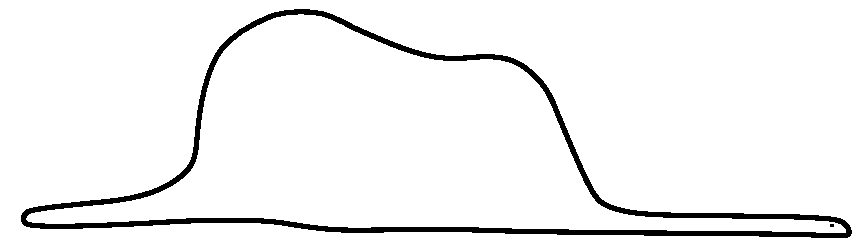
\includegraphics[width=5cm]{vibora-blanca-sola.pdf}
\end{center}

\vfill

\begin{center}
\begin{small}
XLIII Reunión Anual de la Asociación Argentina de Tecnología Nuclear\\
Buenos Aires, Noviembre 2016
\end{small}
\end{center}

\pagebreak

\title{Solving the neutron transport equation by the method of characteristics in milonga neutron code}
\author{Vignolo, R.$^{1}$}
\affiliation{%
$^1$TECNA Estudios y Proyectos de Ingeniería S.A.\\
Encarnaci\'on Ezcurra 365, C1107CLA~Buenos Aires, Argentina\\
\url{rvignolo@tecna.com}\\
}


\maketitle

\selectlanguage{english}
\begin{abstract}
\noindent
Milonga is a neutron code that solves the steady-state multigroup neutron transport equation either by using the diffusion approximation or the discrete ordinates method ($S_N$) over unstructured grids (although simple structured grids can also be used). Both formulations can be solved over a finite-volumes or a finite-elements discretization scheme. Milonga was born as part of a PhD in nuclear engineering and, since it is free software (as in free speech), it may be developed collaboratively by volunteer engineers/computer programmers who do not want to be, as Stamm'ler used to say, users that ``\emph{will never understand the programs they are to use and, as computer slaves, consider them as black boxes, blindy trusting their results''} (Stamm'ler et al., 1983). The implementation of the method of characteristics (MOC) incorporates in milonga a lattice formulation, filling in the missing stage of production calculations: lattice (MOC), lattice-core ($S_N$) and core (diffusion). In this first stage of development of lattice formulations, MOC was selected because it overcome the main limitation for collision probability (CP) method: it does not produce full square matrices of order equal to the number of regions in the domain times the energy groups, so it is possible to solve problems with many more regions. In this context, an efficient ray tracing algorithm for structured and unstructured meshes and a non-linear power method were developed. These two things allow to compute the scalar flux per refion and energy group by collecting all mean angular fluxes over track segments and region sources. This paper discusses about the implementation of the method, preliminary results and future improvements or additions in milonga.
\end{abstract}

\vfill

\begin{center}
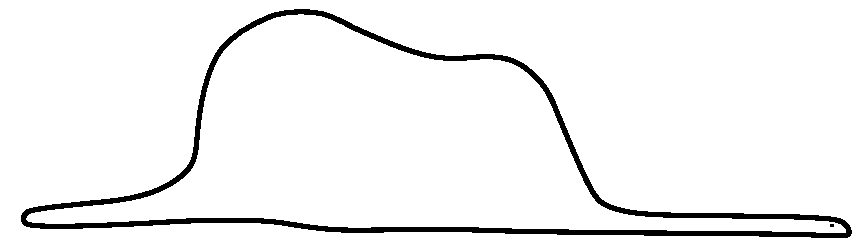
\includegraphics[width=5cm]{vibora-blanca-sola.pdf}
\end{center}

\vfill

\begin{center}
\begin{small}
XLIII Reunión Anual de la Asociación Argentina de Tecnología Nuclear\\
Buenos Aires, November 2016
\end{small}
\end{center}

\addtolength{\textheight}{-2cm}

\pagebreak

\selectlanguage{spanish}

% nombre de tabla
\renewcommand{\tablename}{Tabla}
\rowcolors{1}{black!10}{black!0}

\tableofcontents
\pagebreak


\section{Introducción}

Los cálculos de celda se corresponden, tradicionalmente, con el primer paso del análisis determinístico de reactores. En esta instancia, una celda representativa es resuelta mediante una formulación que pueda ser correctamente aplicada al dominio. Entre estas formulaciones, usualmente se utilizan tanto el método de las probabilidades de colisión (que puede estar asociado al método de las corrientes en las interfaces) como el método de las características. La resolución de la ecuación de transporte en este dominio resulta en la obtención del flujo escalar en una discretización fina en energía y regiones que, posteriormente, es empleada para calcular secciones eficaces homogeneizadas tanto en energía como en el espacio a utilizar como entradas en cálculos de núcleo.

En un comienzo, la celda elemental consistía en un \emph{pin cell} donde sólo se representa una única barra combustible junto al moderador que la rodea y condiciones de contorno reflectivas. Debido al incremento en el poder de cálculo, hoy en día es posible realizar cálculos de celda a nivel de elemento combustible e incluso se busca realizarlos a nivel de núcleo. El método de las características (comúnmente denominado MOC) pareciera ofrecer esta posibilidad, y es por este motivo que durante los últimos años ha ganado un particular interés. 

Milonga es un código neutrónico de núcleo escrito como \emph{plugin} de wasora~\cite{wasora}. Con la incorporación del método de las características como formulación de transporte en 2D se ha abierto el panorama a los cálculos de celda. En este trabajo se describe la implementación de MOC 2D y se presentan algunos resultados preliminares. Por último, se hará un breve hincapié en futuras incorporaciones.


\section{Método de las Características}

MOC resuelve la forma característica de la ecuación de transporte recorriendo lineas rectas (denominadas rayos o \emph{tracks}) que simulan la trayectoria de neutrones a medida que se mueven por el dominio. Este método se basa en la resolución iterativa del flujo a partir de la resolución de la ecuación de transporte sobre dichos \emph{tracks} trazados. El método de las características es generalmente aplicado sobre la forma multigrupo de la ecuación de transporte y sobre dominios compuestos por regiones con propiedades nucleares uniformes. Posteriormente, el flujo escalar de cada región y grupo es computado a partir de la variación del flujo angular sobre cada uno de los \emph{tracks} y de la fuente. 

\subsection{Discretización y nomenclatura}

Debido a la gran cantidad de notación disponible en la bibliografía, es conveniente definir adecuadamente la discretización a utilizar en este trabajo previo a ingresar a la descripción del método. Las diferentes definiciones que se dan a continuación se encuentran representadas gráficamente en la figura~\ref{fig:coords-indices}. En este contexto, se definen:

\begin{itemize}
\renewcommand\labelitemi{$\cdot$}
 \item $g$: índice asociado a un grupo de energía;
 \item $i$: índice asociado a una región con flujo plano;
 \item $m$: índice asociado a un ángulo s\'olido $\boldsymbol{\hat{\Omega}}_m$ (cada índice $m$ tiene asociado un único par de índices $a$ y $p$, que son detallados a continuación);
 \item $a$: índice asociado a un ángulo azimutal $\varphi_a$;
 \item $p$: índice asociado a un ángulo polar $\theta_p$; y
 \item $k$: índice asociado a un segmento de un \emph{track}; $k$ generalmente viene acompañado de los índices $i$ y $m$ para representar los segmentos contenidos en la región $i$ con ángulo $\boldsymbol{\hat{\Omega}}_m$.
\end{itemize}

\begin{figure}[!ht]
 \begin{center}
  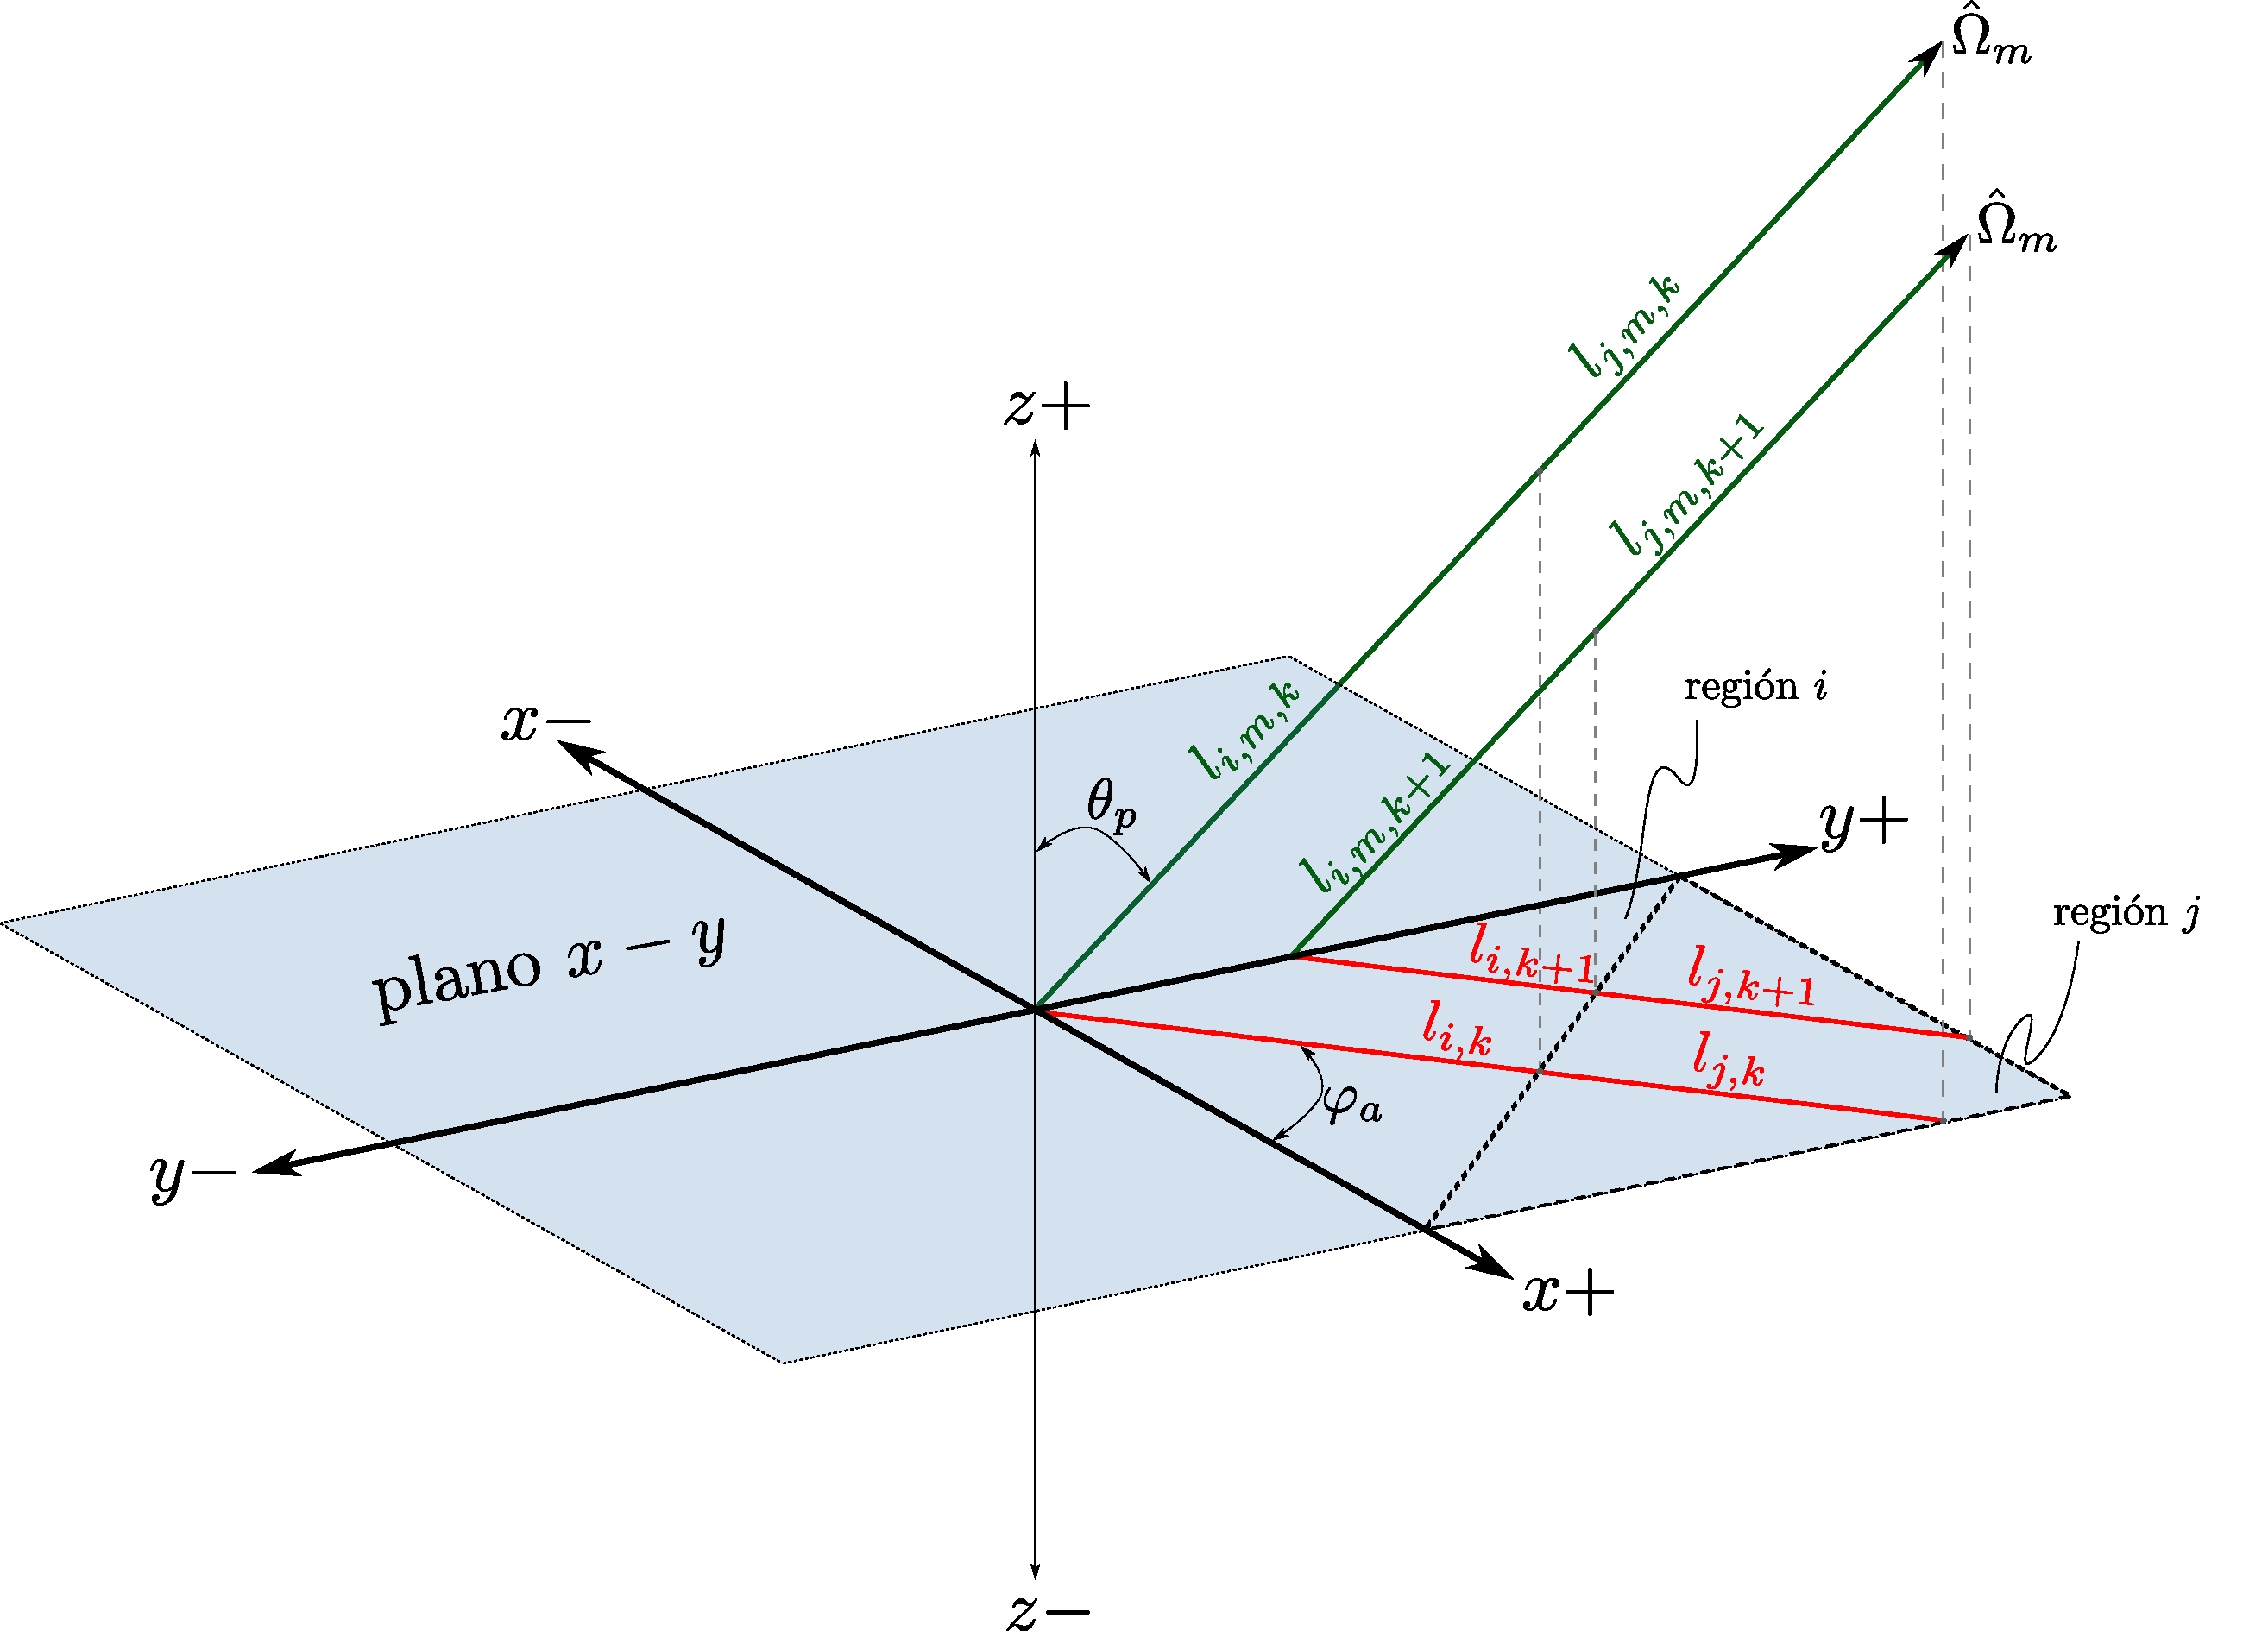
\includegraphics[width=1.0\linewidth]{coords-indices-2.pdf}
 \end{center}
\caption{\label{fig:coords-indices} Discretización espacial de la formulación MOC.}
\end{figure}

Por otra parte, las secciones eficaces responden a la nomenclatura usual:

\begin{itemize}
\renewcommand\labelitemi{$\cdot$}
 \item $\Sigma^s_{g^\prime \rightarrow g}$: sección eficaz de \emph{scattering} de grupo $g^\prime$ a $g$;
 \item $\Sigma^t_g$: sección eficaz total de grupo $g$;
 \item $\Sigma^a_g$: sección eficaz de absorción de grupo $g$; y
 \item $\Sigma^f_g$: sección eficaz de fisión de grupo $g$; y
 \item $\nu$: número de neutrones por fisión.
\end{itemize}

Finalmente, se listan algunas definiciones usuales y otras específicas a MOC:

\begin{itemize}
\renewcommand\labelitemi{$\cdot$}
 \item $\psi^{\text{in}}_{i,g,m,k}$: flujo angular de entrada al segmento $k$ correspondiente a la región $i$, grupo $g$ y ángulo $\boldsymbol{\hat{\Omega}}_m$;
 \item $\psi^{\text{out}}_{i,g,m,k}$: flujo angular de salida del segmento $k$ correspondiente a la región $i$, grupo $g$ y ángulo $\boldsymbol{\hat{\Omega}}_m$;
 \item $\phi_{i,g}$: flujo escalar de la región $i$ y grupo $g$;
 \item $q_{i,g,m}$: fuente angular de la región $i$ y grupo $g$ con dirección $\hat{\Omega}_m$. Para \emph{scattering} isotrópico, $q_{i,g,m} = \frac{1}{4\pi}Q_{i,g}$, donde $Q_{i,g}$ es la fuente de la región $i$ y grupo $g$. De esta forma, $q_{i,g,m}$ es independiente del índice $m$, motivo por el cual se utiliza $q_{i,g,m} = q_{i,g}$.
 \item $l_{i,m,k}$: longitud del segmento $k$ con dirección angular $m$ dentro de la región $i$. Observando la figura~\ref{fig:coords-indices}, la igualdad $l_{i,m,k} = \frac{l_{i,k}}{\sin \theta_p}$ resulta obvia.
\end{itemize}

\subsection{Formulación}

La formulación multigrupo de la ecuación de transporte integro-diferencial estacionaria es~\cite{henry,lamarsh,duderstadt,glasstone,lewis,stammler,handbook-ingnuclear}

\begin{equation}
 \label{eq:transportemultigrupo}
 \boldsymbol{\hat{\Omega}} \cdot \text{grad} \left[ \psi_g(\vec{x}, \boldsymbol{\hat{\Omega}}) \right]
 + \Sigma^t_g(\vec{x}) \cdot \psi_g(\vec{x}, \boldsymbol{\hat{\Omega}}) = q_g(\vec{x}, \boldsymbol{\hat{\Omega}}),
\end{equation}

\noindent
donde, para el caso sin fuentes externas, el término de fuente posee las contribuciones de fisión (isotrópica) y \emph{scattering}

\begin{equation} \label{eq:fuentemultigrupo-1}
 q_g(\vec{x}, \boldsymbol{\hat{\Omega}}) =
 \sum_{g^\prime=1}^G \int_{4\pi} \Sigma^s_{g^\prime \rightarrow g}(\vec{x}, \boldsymbol{\hat{\Omega}^\prime} \rightarrow \boldsymbol{\hat{\Omega}}) \cdot \psi_{g^\prime}(\vec{x}, \boldsymbol{\hat{\Omega}^\prime}) \, d\boldsymbol{\hat{\Omega}^\prime} 
 + \frac{\chi_g}{4\pi k_{\text{eff}}} \sum_{g^\prime=1}^G \int_{4\pi} \nu\Sigma^f_{g^\prime}(\vec{x}) \cdot \psi_{g^\prime}(\vec{x}, \boldsymbol{\hat{\Omega}^\prime}) \, d\boldsymbol{\hat{\Omega}^\prime}.
\end{equation}

\noindent
Suponiendo \emph{scattering} isotrópico y utilizando la definición del flujo escalar a partir del flujo angular se pierde la dependencia con la dirección angular $\boldsymbol{\hat{\Omega}}$ y se obtiene

\begin{equation} \label{eq:fuentemultigrupo-2}
 q_g(\vec{x}, \boldsymbol{\hat{\Omega}}) = 
 q_g(\vec{x}) = 
 \frac{1}{4\pi} \left(
 \sum_{g^\prime=1}^G \Sigma^s_{g^\prime \rightarrow g}(\vec{x}) \cdot \phi_{g^\prime}(\vec{x})
 + \frac{\chi_g}{k_{\text{eff}}} \sum_{g^\prime=1}^G \nu\Sigma^f_{g^\prime}(\vec{x}) \cdot \phi_{g^\prime}(\vec{x}) 
 \right).
\end{equation}

Aplicando MOC a la ecuación de transporte multigrupo~\eqref{eq:transportemultigrupo} se obtiene una ecuación diferencial lineal de primer orden~\cite{glasstone,handbook-ingnuclear}

\begin{equation} \label{eq:caracteristica}
 \frac{d}{ds}\psi_g(\vec{r_0}+s\boldsymbol{\hat{\Omega}},\boldsymbol{\hat{\Omega}}) 
 + \Sigma^t_g(\vec{r_0}+s\boldsymbol{\hat{\Omega}}) \cdot \psi_g(\vec{r_0}+s\boldsymbol{\hat{\Omega}}, \boldsymbol{\hat{\Omega}}) = 
 q_g(\vec{r_0}+s\boldsymbol{\hat{\Omega}})
\end{equation}

\noindent
que será aplicada a cada segmento de cada \emph{track} trazado sobre la geometría a analizar. Estas líneas responden a la ecuación $\vec{r_0}+s\boldsymbol{\hat{\Omega}}$, donde $s$ es la distancia al punto $\vec{r_0}$ medida sobre la dirección $\boldsymbol{\hat{\Omega}}$. Como se verá a continuación, realizando un \emph{ray tracing} sobre la geometría del problema a partir de la selección de diferentes puntos de inicio $\vec{r_0}$ y direcciones $\boldsymbol{\hat{\Omega}}$ y resolviendo la ecuación característica~\eqref{eq:caracteristica} sobre cada uno de los segmentos de cada \emph{tracks}, es posible obtener la información necesaria para la determinación del flujo escalar en cada región y grupo de energía. Al discretizar la ecuación~\eqref{eq:caracteristica} y aplicar la notación descripta para este trabajo, se obtiene

\begin{equation} \label{eq:edo-disc}
 \frac{d}{ds}\psi_{i,g,m,k} (s)
 + \Sigma^t_{i,g} \cdot \psi_{i,g,m,k} (s) = 
 q_{i,g,m}
\end{equation}

\noindent
donde además se ha asumido la aproximación de fuente plana en cada región y por este motivo $q$ ha perdido la dependencia con $s$, resultando en

\begin{equation} \label{eq:fuente-isotropica}
 q_{i,g,m} = q_{i,g} = 
 \frac{1}{4\pi} \left(
 \sum_{g^\prime=1}^G \Sigma^s_{i,g^\prime \rightarrow g} \cdot \phi_{i,g^\prime}
 + \frac{\chi_g}{k_{\text{eff}}} \sum_{g^\prime=1}^G \nu\Sigma^f_{i,g^\prime} \cdot \phi_{i,g^\prime}
 \right).
\end{equation}

La ecuación~\eqref{eq:edo-disc} puede ser resuelta para cada segmento de cada \emph{track}, siempre y cuando se conozca la condici\'on inicial. En particular, el resultado para el flujo angular a la salida de un segmento es

\begin{equation}
 \psi^{\text{out}}_{i,g,m,k} = \psi^{\text{in}}_{i,g,m,k} \cdot e^{-\tau_{i,g,m,k}}
 + \frac{q_{i,g}}{\Sigma^t_{i,g}} \left(1 - e^{-\tau_{i,g,m,k}} \right),
\end{equation}

\noindent
siendo $\tau_{i,g,m,k}$ el camino óptico, definido como el producto $l_{i,m,k} \cdot \Sigma^t_{i,g}$. Reacomodando, la variación del flujo angular en un segmento puede escribirse como

\begin{equation} \label{eq:delta-psi}
 \Delta \psi_{i,g,m,k} = 
 \psi^{\text{in}}_{i,g,m,k} - \psi^{\text{out}}_{i,g,m,k} = 
 \left( \psi^{\text{in}}_{i,g,m,k} - \frac{q_{i,g}}{\Sigma^t_{i,g}} \right) \left(1 - e^{-\tau_{i,g,m,k}} \right).
\end{equation}

El valor medio del flujo angular del segmento $k$ correspondiente a la región $i$, grupo $g$ y dirección $\boldsymbol{\hat{\Omega}}_m$ se obtiene integrando la soluci\'on de la ecuación~\eqref{eq:edo-disc} de la siguiente forma

\begin{multline}
 \overline{\psi}_{i,g,m,k} =
 \frac{1}{l_{i,m,k}} \int_{s_{\text{in}}}^{s_{\text{out}}} \psi_{i,g,m,k} (s) \, ds = \\
 \frac{1}{l_{i,m,k}} \left[ \frac{\psi^{\text{in}}_{i,g,m,k}}{\Sigma^t_{i,g}} \left(1 - e^{-\tau_{i,g,m,k}} \right) + \frac{l_{i,m,k} \cdot q_{i,g}}{\Sigma^t_{i,g}} \left( 1 - \frac{\left(1 - e^{-\tau_{i,g,m,k}} \right)}{\tau_{i,g,m,k}} \right) \right].
\end{multline}

\noindent
Luego, utilizando el resultado de la ecuación~\eqref{eq:delta-psi} sobre la expresi\'on del flujo angular medio, se obtiene

\begin{equation} \label{eq:flujo-ang-medio-en-segmento}
 \overline{\psi}_{i,g,m,k} = \frac{q_{i,g}}{\Sigma^t_{i,g}} + \frac{\Delta \psi_{i,g,m,k}}{\tau_{i,g,m,k}}.
\end{equation}

El flujo angular medio en la región $i$, grupo $g$ y dirección $\boldsymbol{\hat{\Omega}}_m$ puede ser obtenido a partir de la contribuci\'on de cada segmento $k$ en la región $i$

\begin{equation} \label{eq:flujo-ang-medio-en-region}
 \overline{\psi}_{i,g,m} = \frac{\sum_{k \in K(i,m)} \overline{\psi}_{i,g,m,k} l_{i,k} \delta_m}{\sum_{k \in K(i,m)} l_{i,k} \delta_m},
\end{equation}

\noindent
donde $k \in K(i,m)$ representa los segmentos correspondientes a una región $i$ con dirección $\boldsymbol{\hat{\Omega}}_m$ y $\delta_m$ la separaci\'on entre segmentos para un dado ángulo azimutal especificado en $\boldsymbol{\hat{\Omega}}_m$. Para encontrar al flujo escalar en una región $i$ y a un grupo $g$, basta con integrar en ángulo s\'olido la expresi\'on obtenida en~\eqref{eq:flujo-ang-medio-en-region} de la siguiente manera

\begin{equation} \label{eq:flujo-escalar-1}
 \phi_{i,g} = \int_{4\pi} \overline{\psi}_{i,g} (\boldsymbol{\hat{\Omega}}) \, d\boldsymbol{\hat{\Omega}} \approx 
 4\pi \sum_m w_m \overline{\psi}_{i,g,m}.
\end{equation}

\noindent
En este caso, $w_m$ son los pesos de la cuadratura angular normalizados, de forma que $\sum_m w_m = \sum_a \sum_p w_a w_p = \sum_a w_a \sum_p w_p = 1$. En primera instancia, es necesario implementar el resultado obtenido en la ecuación~\eqref{eq:flujo-ang-medio-en-region} en~\eqref{eq:flujo-escalar-1}

\begin{equation} \label{eq:flujo-escalar-2}
 \phi_{i,g} =
 4\pi \sum_m \left( w_m \frac{\sum_{k \in K(i,m)} \overline{\psi}_{i,g,m,k} l_{i,k} \delta_m}{\sum_{k \in K(i,m)} l_{i,k} \delta_m} \right) = 
 \frac{4\pi}{A_i} \sum_m \left( w_m \delta_m \sum_{k \in K(i,m)} \overline{\psi}_{i,g,m,k} l_{i,k} \right).
\end{equation}

\noindent
En la anterior ecuación puede verse que el t\'ermino $A_{i,m} = \sum_{k \in K(i,m)} l_{i,k} \delta_m = \delta_m \sum_{k \in K(i,m)} l_{i,k}$ representa el área de la región $i$ computada a partir de los segmentos $l_{i,k}$ (proyectados sobre el plano $x - y$) y con ángulo azimutal contenido en $\boldsymbol{\hat{\Omega}}_m$. En un \emph{ray tracing} con la suficiente densidad de lineas puede suponerse que el área obtenida a partir de esta expresi\'on es independiente de la dirección azimutal de los segmentos, motivo por el cual $A_{i,m} = A_i$ y es retirado de la sumatoria sobre $m$.

Por último, la expresi\'on para el flujo escalar puede simplificarse aún m\'as incorporando el resultado de la ecuación~\eqref{eq:flujo-ang-medio-en-segmento} sobre~\eqref{eq:flujo-escalar-2}

\begin{multline} \label{eq:flujo-escalar-3}
 \phi_{i,g} =
 \frac{4\pi}{A_i} \sum_m \left\lbrace w_m \delta_m \sum_{k \in K(i,m)} \left[ l_{i,k} \left( \frac{q_{i,g}}{\Sigma^t_{i,g}} + \frac{\Delta \psi_{i,g,m,k}}{\tau_{i,g,m,k}} \right) \right] \right\rbrace \\ 
 = \frac{4\pi}{A_i} \cdot \frac{q_{i,g}}{\Sigma^t_{i,g}} \sum_m \left( w_m \delta_m \sum_{k \in K(i,m)} l_{i,k} \right) + \frac{4\pi}{A_i \cdot \Sigma^t_{i,g}} \sum_m \left( w_m \delta_m \sin \theta_p \sum_{k \in K(i,m)} \Delta \psi_{i,g,m,k} \right) \\ 
 = \frac{4\pi}{\Sigma^t_{i,g}} \left[ q_{i,g} + \frac{1}{A_i} \sum_m \left( w_m \delta_m \sin \theta_p \sum_{k \in K(i,m)} \Delta \psi_{i,g,m,k} \right) \right]
 .
\end{multline}

La resolución de las ecuaciones~\eqref{eq:fuente-isotropica}, \eqref{eq:delta-psi} y~\eqref{eq:flujo-escalar-3} permiten obtener la distribución espacial y energética del flujo escalar. Sin embargo, el proceso es iterativo hasta que los criterios de convergencia del flujo, fuentes, condiciones de contorno y valor de $k_{\text{eff}}$ sean satisfechos. Comúnmente, el nombre atribuido a cada una de estas iteraciones se conoce como \emph{transport sweep}. En cada \emph{transport sweep} se calcula el flujo escalar con~\eqref{eq:flujo-escalar-3} a partir de las contribuciones del flujo angular sobre cada región y grupo obtenidas mediante~\eqref{eq:delta-psi}. Posteriormente se computa el factor de multiplicación y se actualizan los valores de las fuentes $q_{i,g}$ seg\'un \eqref{eq:fuente-isotropica}.

Por completitud, convienen detallar las cuadraturas azimutales y polares que pueden utilizarse para aproximar la integral sobre \'angulo s\'olido. Se ha decido normalizar los pesos $w_m$, de forma que $\sum_a w_a = 1$ y $\sum_p w_p = 1$. En cuanto a la cuadratura azimutal, la forma más simple de obtener cada ángulo $\varphi_a$ es dividiendo el dominio azimutal en ángulos equiespaciados:

\begin{equation}
 \Delta \varphi_a = \frac{2\pi}{A},
\end{equation}

\noindent
siendo $A$ el número total de ángulos azimutales. Sin embargo, como se verá en la sección~\ref{sec:ray-tracing}, pequeñas correcciones sobre cada $\varphi_a$ deben ser realizadas con el fin de realizar un \emph{ray tracing} cíclico. Milonga elige cada ángulo azimutal $\varphi_a$ con $a \in \left\lbrace 0, 1, ..., A-1 \right\rbrace$ mediante

\begin{equation}
 \varphi_a = \frac{2\pi}{A} \left( a + \frac{1}{2} \right).
\end{equation}

\noindent
Posteriormente, cada ángulo $\varphi_a$ se corrige de forma tal que el \emph{ray tracing} sea cíclico. Luego, el peso asociado a $\varphi_a$ se obtiene a partir de

\begin{equation}
 w_a = \frac{1}{4\pi} \left( \varphi_{a+1} - \varphi_{a-1} \right).
\end{equation}

Milonga trabaja con diferentes cuadraturas polares descriptas, en su mayoría, en~\cite{handbook-ingnuclear} y~\cite{tabuchi}. Entre ellas, es posible hacer uso de cuadraturas tipo \emph{equal angle}, \emph{equal weight}, Gauss-Legendre, Leonard y Tabuchi-Yamamoto (seleccionada por defecto).

\section{Geometr\'ias en milonga}

Las geometrias en milonga se interpretan a traves de mallas, ya sean estructuradas o no estructuradas. 

caso particular de moc: tienen que ser un dominio rectangular, pero oprque es así lo explico mas adelante.

\subsection{Mallas estructuradas y no estructuradas}

\subsection{\emph{Ray tracing} de mallas 2D} \label{sec:ray-tracing}

La realizaci\'on del \emph{ray tracing} sobre la geometría del problema a resolver es uno de los pasos más importantes que debe afrontarse en el método de las características. Luego de este procedimiento, se dispone de las estructuras de datos que almacenan información de los \emph{tracks}, principalmente los segmentos que los forman y la región a la que cada uno de ellos pertenece. Como se ha visto anteriormente, la actual formulación MOC implementada en milonga acepta únicamente dominios rectangulares. El motivo de esta limitación radica en que el tipo de algoritmo de \emph{ray tracing} desarrollado es de tipo c\'iclico, tal como puede verse en la figura~\ref{fig:cyclic-tracks} y se describe a continuación. Por simetr\'ia, solo es necesario trazar \emph{tracks} con $\varphi \in \left[ 0, \pi \right]$ debido a que aquellos con $\varphi + \pi$ poseen los mismos puntos de definición. Por otro lado, los \emph{tracks} con ángulos azimutales suplementarios tienen un espaciado tal que forman recorridos cerrados. En conclusión, para realizar un trazado de \emph{tracks} en un dominio de estas características, solo es necesario conocer las dimensiones de la \emph{bounding box} de la geometría y datos de entrada: densidad o espaciado de líneas y número de ángulos azimutales.

\begin{figure}[!ht]
 \begin{center}
  \subfloat[\label{fig:cyclic-tracks-1}]{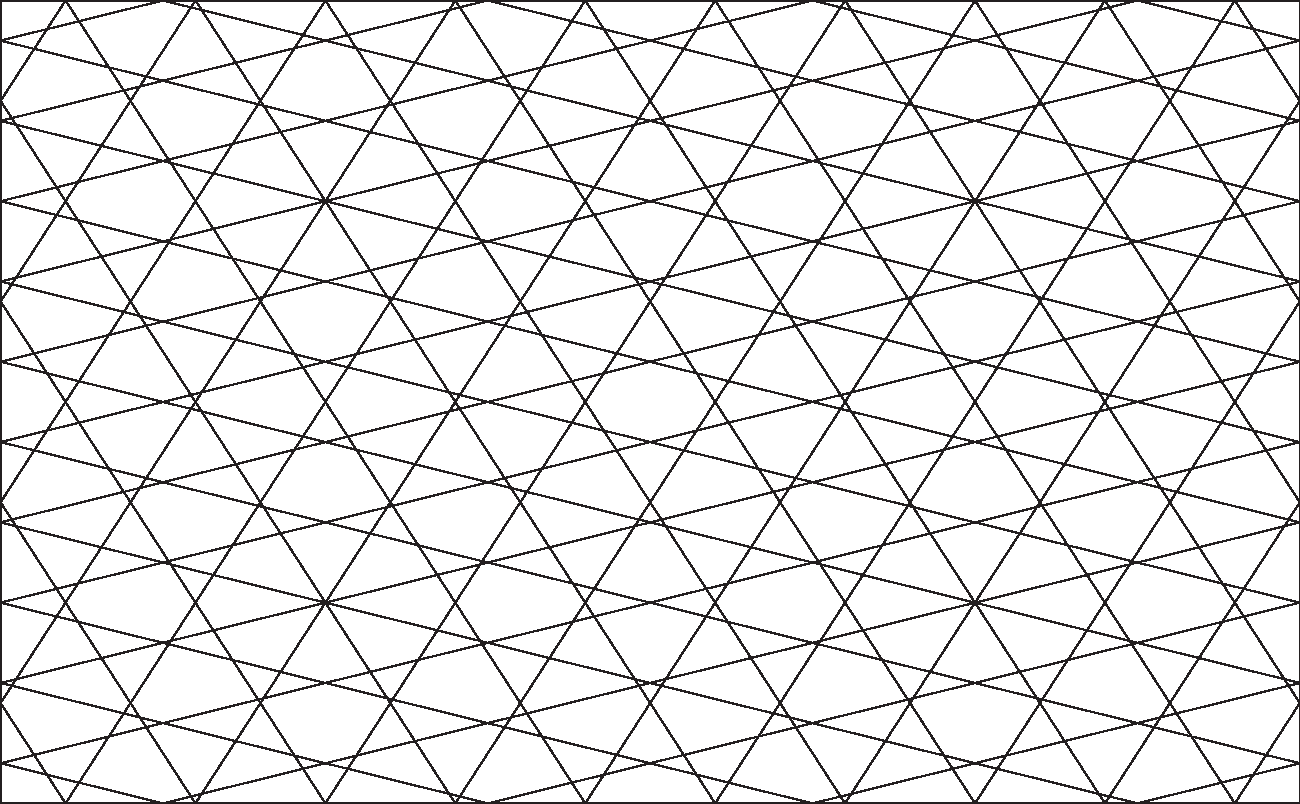
\includegraphics[width=0.485\linewidth]{graficos/cyclic-tracks/cyclic-tracks-1.pdf}} 
  \subfloat[\label{fig:cyclic-tracks-2}]{ 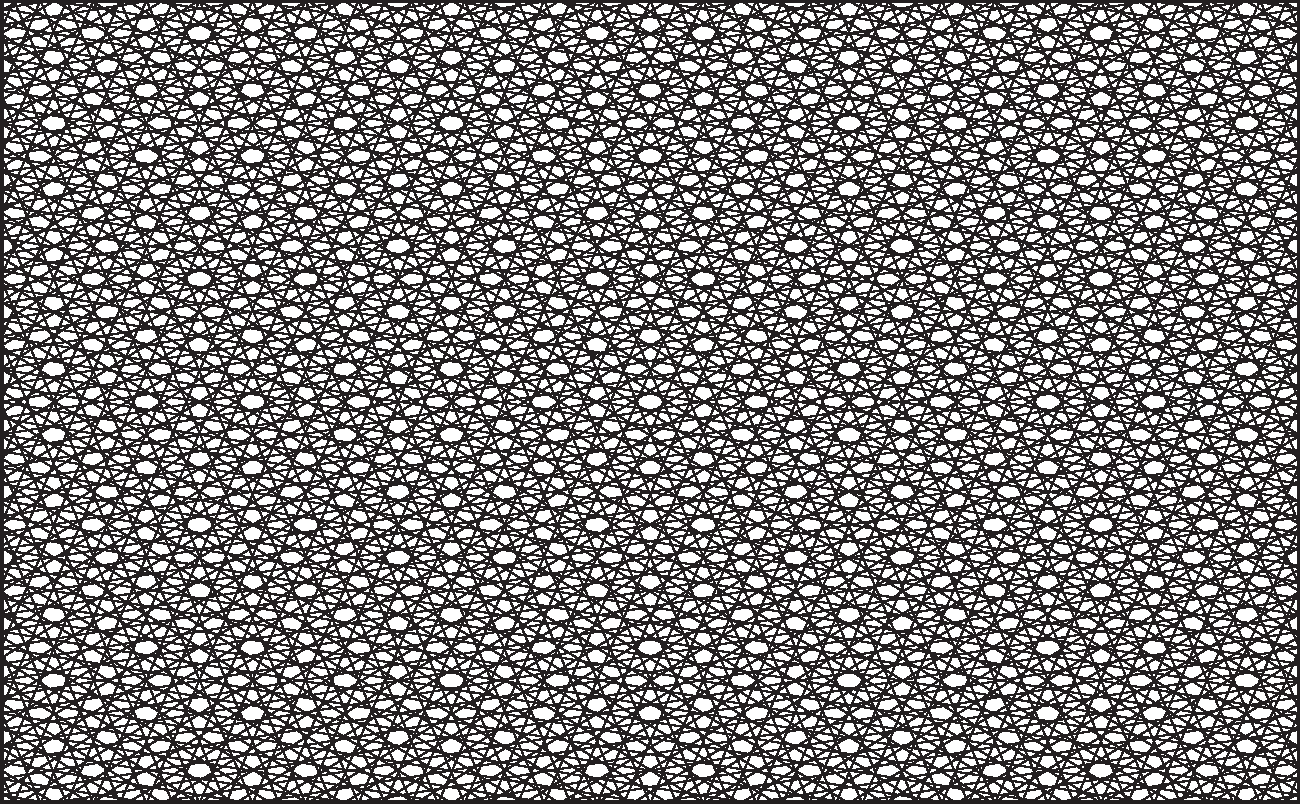
\includegraphics[width=0.485\linewidth]{graficos/cyclic-tracks/cyclic-tracks-2.pdf}}\\
  \caption{\emph{Tracks} de dos \emph{ray tracing} cíclicos trazados sobre un dominio rectangular. La figura~\ref{fig:cyclic-tracks-1} permite visualizar el mecanismo del trazado de líneas, mientras que la figura~\ref{fig:cyclic-tracks-2} demuestra el resultado obtenido al aplicar el mismo procedimiento pero considerando una mayor discretización en ángulos azimutales y densidad de líneas.}
  \label{fig:cyclic-tracks}
 \end{center}
\end{figure}

La principal ventaja de utilizar \emph{cyclic tracking} es el manejo de las condiciones de contorno debido a que no es necesario realizar aproximaciones de ningún tipo. Si la condición de contorno es de vacío, el flujo angular entrante a determinado \emph{track} es simplemente nulo. Para los casos con condiciones de contorno reflectivas o periódicas, el flujo angular entrante a cada \emph{track} es igual al flujo angular saliente de algún otro (dependiendo la condición de contorno). En este sentido, milonga conecta adecuadamente los \emph{tracks}.

Una vez definidos los \emph{tracks}, es momento de discretizarlos en segmentos correspondientes a cada región que atraviesan y así obtener la información necesaria para computar las variaciones del flujo angular a partir de la ecuación~\eqref{eq:delta-psi}. En la figura~\ref{fig:mesh-and-segments-1} se presentan, por un lado un mallado conformado mediante \emph{delaunay} y, por el otro, los segmentos coloreados por región resultantes de un \emph{ray tracing}. En este caso, la espaciado entre líneas y número de ángulos $\varphi$ seleccionados no permiten distinguir los segmentos graficados. Por este motivo, en la figura~\ref{fig:mesh-and-segments-2} se presenta el \emph{ray tracing} sobre una malla con elementos recombinados a partir de la malla en~\ref{fig:mesh-1} y parámetros de \emph{tracking} que permiten visualizar los segmentos de forma individual.

\begin{figure}[!ht]
 \begin{center}
  \subfloat[\label{fig:mesh-1}]{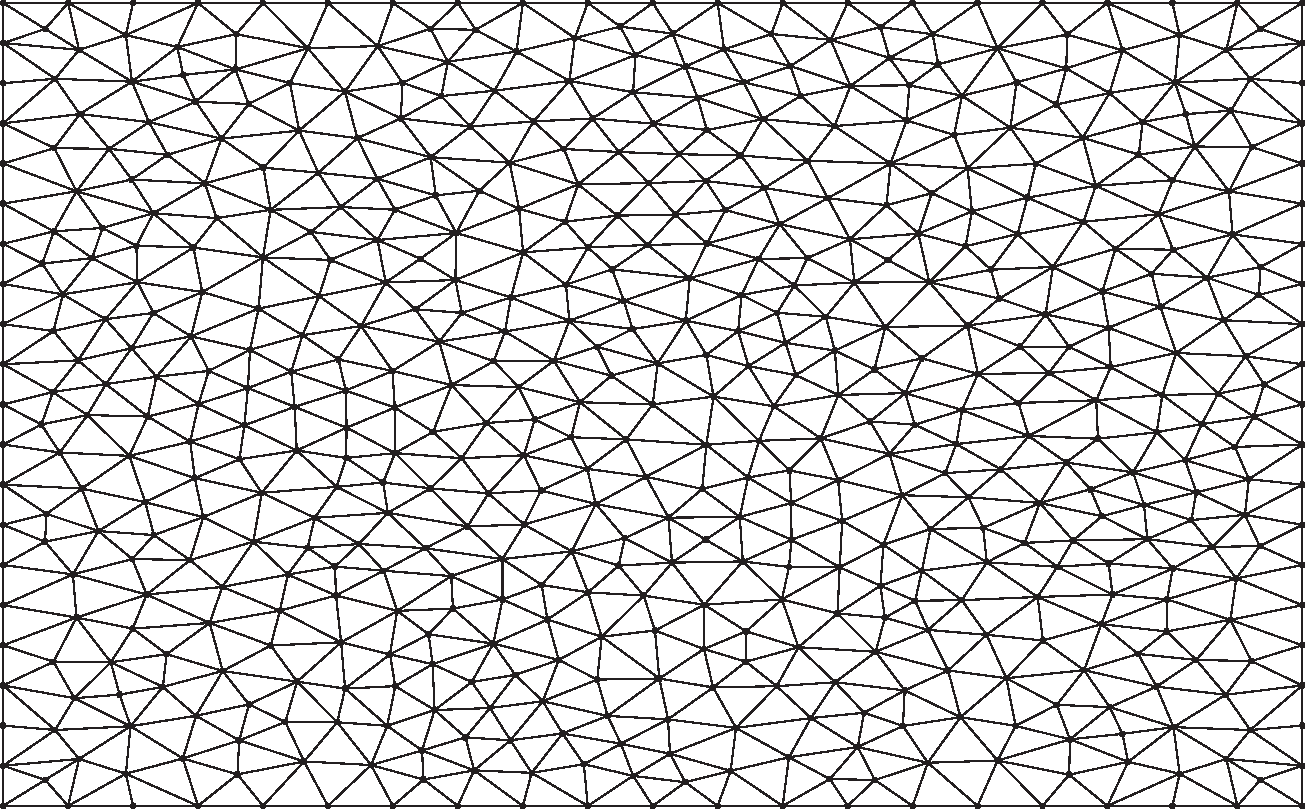
\includegraphics[width=0.479\linewidth]{graficos/meshes-and-segments/mesh-1.pdf}} 
  \subfloat[\label{fig:segments-1}]{ 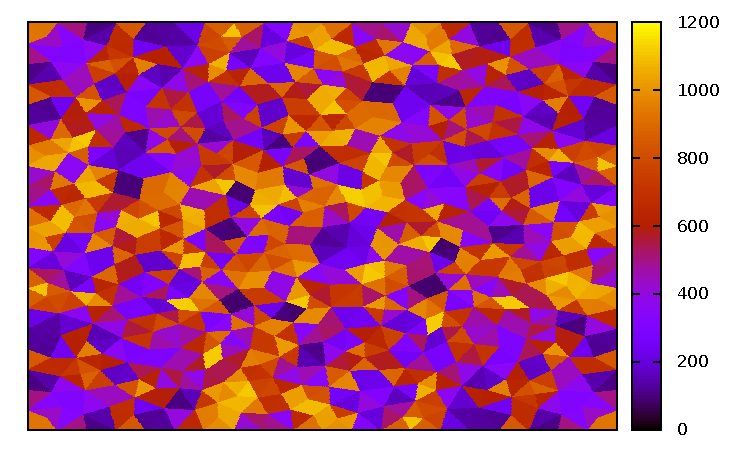
\includegraphics[width=0.501\linewidth]{graficos/meshes-and-segments/segments-1.pdf}}\\
  \caption{(\ref{fig:mesh-1}) presenta la malla de un determinado problema y~(\ref{fig:segments-1}) la segmentación de los \emph{tracks} sobre la misma. No es posible visualizar los segmentos de forma independiente debido a la cantidad de ángulos $\varphi$ y separación de líneas seleccionada.}
  \label{fig:mesh-and-segments-1}
 \end{center}
\end{figure}

\begin{figure}[!ht]
 \begin{center}
  \subfloat[\label{fig:mesh-2}]{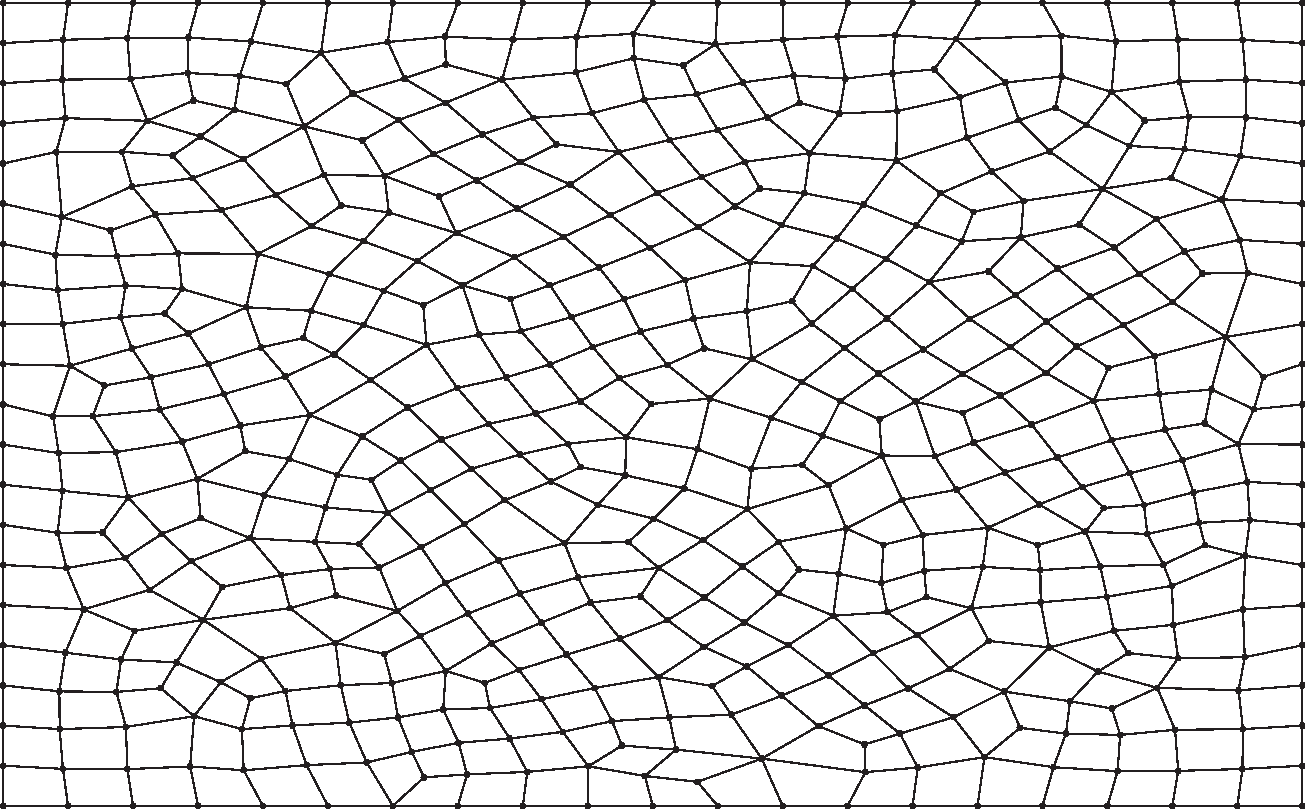
\includegraphics[width=0.479\linewidth]{graficos/meshes-and-segments/mesh-2.pdf}}
  \subfloat[\label{fig:segments-2}]{ 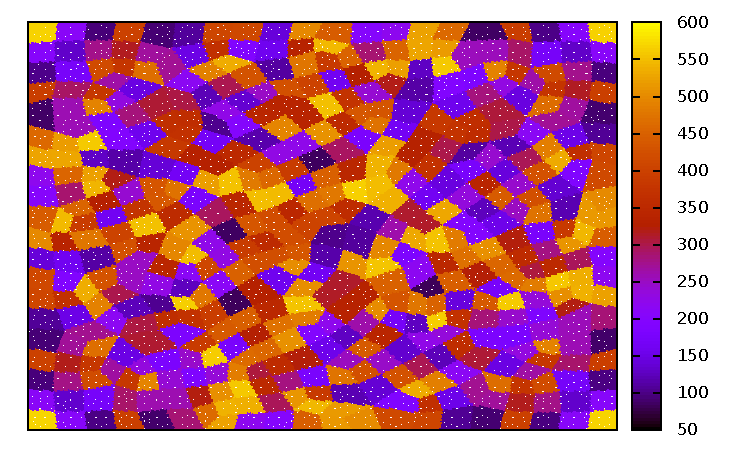
\includegraphics[width=0.501\linewidth]{graficos/meshes-and-segments/segments-2.pdf}}\\
  \caption{Con el fin de demostrar la capacidad de realizar \emph{ray tracings} sobre diferentes elementos y, además, poner en evidencia los segmentos no visibles en la figura~\ref{fig:segments-1}, se presentan las figuras~\ref{fig:mesh-2} y~\ref{fig:segments-2}.}
  \label{fig:mesh-and-segments-2}
 \end{center}
\end{figure}

Opcionalmente, milonga efectúa la comparación de las áreas reales de cada región y las computadas a partir del \emph{tracking} de la malla, indicando si es necesario modificar sus parámetros. Por otro lado, la evaluación de la función exponencial de la ecuación~\eqref{eq:delta-psi} puede ser sustituida por una aproximación lineal por partes, requiriendo eventualmente la segmentación de segmentos dentro de una misma región ya que se podría incurrir en errores mayores a los deseados~\cite{openmoc2014}.


\section{MOC \emph{solver}}

En esta sección se darán algunos detalles del algoritmo que resuelve la formulación de transporte a través del método de las características en milonga. En cada \emph{transport sweep} se calcula $\phi_{i,g}$ a partir de la ecuaci\'on~\eqref{eq:flujo-escalar-3}. Como se mencion\'o previamente, la sumatoria sobre $k \in K(i,m)$ hace referencia a los segmentos que la atraviesan con dirección $\boldsymbol{\hat{\Omega}}_m$ la región $i$, por lo que una forma de obtener $\phi_{i,g}$ es recorrer cada \emph{track} contabilizando el aporte a $\phi_{i,g}$ de cada segmento. La figura~\ref{fig:tracks-solver} representa el orden en que milonga recorre cada segmento de cada \emph{track}. En este contexto, la ecuaci\'on~\eqref{eq:flujo-escalar-3} es resuelta para el primer segmento del \emph{track} señalado en el primer recuadro a partir de un \emph{guess} inicial de flujo angular entrante. El aporte de este segmento al flujo escalar es contabilizado y almacenado. Posteriormente, se contin\'ua con el recorrido del \emph{track} hacia delante hasta llegar a la frontera del dominio. Luego, el mismo \emph{track} es recorrido en sentido inverso\footnote{Es importante tener en cuenta que antes de recorrer el \emph{track} en sentido contrario también se realizan los recorridos para cada \'angulo polar $p$ y grupo de energía $g$.}. El proceso se repite para todas las l\'ineas de trazo con una misma dirección azimutal y, dependiendo de la condición de contorno, el flujo angular saliente de un \emph{track} es considerado como flujo angular entrante del que corresponda en un \emph{transport sweep} posterior. Una vez que se finaliza con los rayos de determinada dirección azimutal, se procede con los pertenecientes a otra y se repite la misma l\'ogica.

\begin{figure}[!ht]
 \begin{center}
  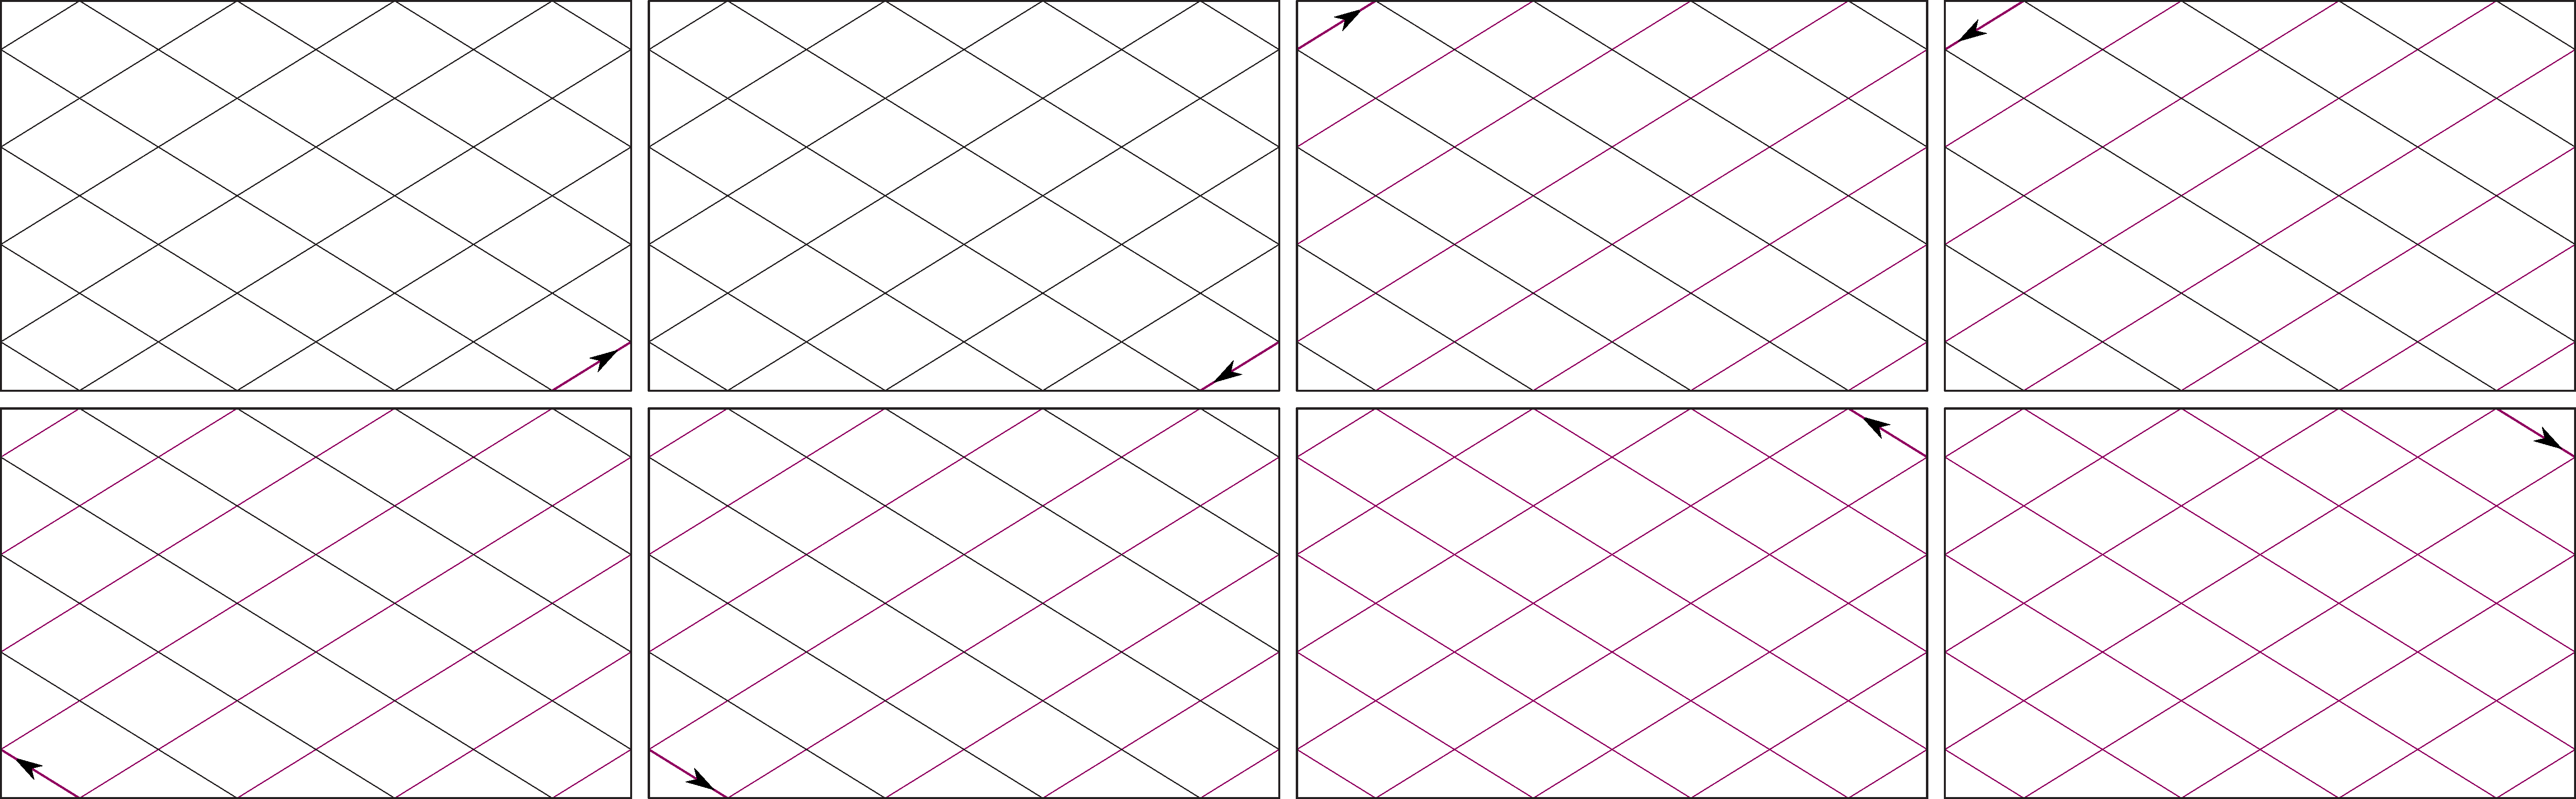
\includegraphics[width=1.0\linewidth]{graficos/solver/cyclic-tracks-1.pdf}
 \end{center}
\caption{\label{fig:tracks-solver} Recorrido de \emph{tracks} en un \emph{transport sweep} de milonga. Los rayos de color se corresponden con aquellos que ya han sido recorridos y las flechas indican el sentido en que se los recorre.}
\end{figure}


\section{Sintaxis}

La intenci\'on de esta secci\'on no es explicar en detalle la sintaxis detr\'as de milonga ya que esto implicar\'ia, necesariamente, escribir acerca de la sintaxis de wasora. Mucho de esto puede ser consultado en las referencias~\cite{wasora, milongabase2010, milonga-db, enief-milonga-2014}, m\'as all\'a de que la documentaci\'on disponible pueda diferir de la actual implementación en milonga. Por otro lado, las consultas a los desarrolladores del c\'odigo son m\'as que bienvenidas. 

La definici\'on de un problema a resolver con el m\'etodo de las características requiere de algunas nuevas consideraciones. En primer lugar, la formulación MOC necesita ser provista de una estructura de \emph{ray tracing}. Milonga permite, en un mismo \emph{input}, generar diferentes estructuras de este tipo sobre una misma o diferentes mallas mediante las siguientes sentencias

\begin{lstlisting}[style=wasora]
TRACK_MESH MESH unstructured N_AZIM_ANGLES 24 TRACK_SPACING 0.02 TINY_STEP 1e-3 NAME track_1 DO_NOT_CHECK_VOLUMES
TRACK_MESH MESH unstructured N_AZIM_ANGLES 32 TRACK_DENS   20.00 TINY_STEP 1e-3 NAME track_2
\end{lstlisting}

\noindent
donde \texttt{N_AZIM_ANGLES} hace referencia al n\'umero de \'angulos azimutales, \texttt{TRACK_SPACING} al espaciado entre l\'ineas, \texttt{TRACK_DENS} a la densidad de l\'ineas por \si{\centi\metre}, \texttt{TINY_STEP} a la magnitud a moverse sobre un \emph{track} para encontrar al elemento vecino y \texttt{DO_NOT_CHECK_VOLUMES} es una palabra clave que en el caso de indicarse se evita contrastar los volúmenes reales de cada elemento con los computados a partir del \emph{ray tracing} realizado. En este caso, dos trazados de l\'ineas se realizaron sobre la misma malla (\texttt{unstructured}) con diferentes par\'ametros, y se almacenaron bajo diferentes nombres: \texttt{track_1} y \texttt{track_2}.

Cada estructura de \emph{ray tracing} tiene definida por defecto una cuadratura polar. Sin embargo, el usuario puede definir distintas cuadraturas polares a trav\'es de

\begin{lstlisting}[style=wasora]
POLAR_QUADRATURE NAME polar_1 N_POLAR_ANGLES 6 TYPE tabuchi_yamamoto
\end{lstlisting}

\noindent
Otras cuadraturas polares disponibles son \texttt{equal_weight}, \texttt{equal_angle}, \texttt{gauss_legendre} y \texttt{leonard}. Por otra parte, el usuario puede proveer las cuadraturas a partir de la \emph{keyword} \texttt{DATA} en reemplazo de \texttt{TYPE}.

Por \'ultimo, al definir el problema a resolver con la formulación MOC, debe proveerse de la estructura de \emph{ray tracing} y, en el caso de ser necesario, la cuadratura polar:

\begin{lstlisting}[style=wasora]
MILONGA_PROBLEM FORMULATION moc TRACK track_1 POLAR_QUADRATURE polar_1 ...
\end{lstlisting}


\section{Resultados}

Si bien la incorporaci\'on del m\'etodo de las características en milonga se encuentra en una etapa de activo desarrollo, se presentan a modo ilustrativo algunos resultados obtenidos por medio de esta herramienta. En este contexto, en primera instancia se realizan dos \emph{benchmarks} de c\'alculo de medio infinito homog\'eneo reportados en~\cite{sood} y luego una celda heterog\'enea de BWR reportada en~\cite{hong} y~\cite{Mazumdar}. Estos c\'alculos permiten poner en evidencia la capacidad de la formulación MOC en milonga.

\subsection{\emph{Benchmarks} de medio homog\'eneo infinito}

Los \emph{benchmarks} presentados en esta sección tienen como fin demostrar que la formulación MOC de milonga, al resolver sobre las l\'ineas de trazo, satisface la relaci\'on de conservaci\'on planteada en la ecuación de transporte~\eqref{eq:transportemultigrupo}. En este caso, es indiferente que geometr\'ia se seleccione para resolver los problemas. Las secciones eficaces de ambos \emph{benchmarks} se detallan en las tablas~\ref{tabla:xs-pua} y~\ref{tabla:xs-urr}, mientras que los resultados obtenidos se listan en la tabla~\ref{tabla:k-infty}. Puede verse la perfecta concordancia con los valores de referencia.

{
\begin{table}[h!]
\begin{center}
\begin{tabular}{cccccccc}
\small \emph{Benchmark}  & \small $g$ & \small $\chi_g$ & \small $\Sigma^{f}_g$ & \small $\nu\Sigma^{f}_g$ & \small $\Sigma^{a}_g$ & \small $\Sigma^{t}_g$ & \small $\Sigma^s_{1 \rightarrow 1}$ \\
\small Pua-1-0-IN & \tiny \num{1} & \tiny \num{1.0} & \tiny \num{0.0816} & \tiny \num{0.264384} & \tiny \num{0.101184} & \tiny \num{0.3264} & \tiny \num{0.225216}
\end{tabular}
\caption{\label{tabla:xs-pua} Secciones eficaces en~\si{\per\centi\metre} para el \emph{benchmark} de medio homogéneo infinito a un grupo de energía.}
\end{center}
\end{table}
}

{
\begin{table}[h!]
\begin{center}
\begin{tabular}{lcccccccccccc}
\small \emph{Benchmark}  & \small $g$ & \small $\chi_g$ & \small $\Sigma^{f}_g$ & \small $\nu\Sigma^{f}_g$ & \small $\Sigma^{a}_g$ & \small $\Sigma^{t}_g$ & \small $\Sigma^s_{g \rightarrow 1}$ & \small $\Sigma^s_{g \rightarrow 2}$ & \small $\Sigma^s_{g \rightarrow 3}$ & \small $\Sigma^s_{g \rightarrow 4}$ & \small $\Sigma^s_{g \rightarrow 5}$ & \small $\Sigma^s_{g \rightarrow 6}$ \\
\small{URR-6-0-IN} & \tiny \num{1} & \tiny \num{0.48} & \tiny \num{0.006} & \tiny \num{0.018} & \tiny \num{0.012} & \tiny \num{0.240} & \tiny \num{0.024} & \tiny \num{0.171} & \tiny \num{0.033} & \tiny \num{0.000} & \tiny \num{0.000} & \tiny \num{0.000} \\
           & \tiny \num{2} & \tiny \num{0.02} & \tiny \num{0.060} & \tiny \num{0.150} & \tiny \num{0.100} & \tiny \num{0.975} & \tiny \num{0.000} & \tiny \num{0.600} & \tiny \num{0.275} & \tiny \num{0.000} & \tiny \num{0.000} & \tiny \num{0.000} \\
           & \tiny \num{3} & \tiny \num{0.00} & \tiny \num{0.900} & \tiny \num{1.800} & \tiny \num{1.100} & \tiny \num{3.100} & \tiny \num{0.000} & \tiny \num{0.000} & \tiny \num{2.000} & \tiny \num{0.000} & \tiny \num{0.000} & \tiny \num{0.000} \\
           & \tiny \num{4} & \tiny \num{0.00} & \tiny \num{0.900} & \tiny \num{1.800} & \tiny \num{1.100} & \tiny \num{3.100} & \tiny \num{0.000} & \tiny \num{0.000} & \tiny \num{0.000} & \tiny \num{2.000} & \tiny \num{0.000} & \tiny \num{0.000} \\
           & \tiny \num{5} & \tiny \num{0.02} & \tiny \num{0.060} & \tiny \num{0.150} & \tiny \num{0.100} & \tiny \num{0.975} & \tiny \num{0.000} & \tiny \num{0.000} & \tiny \num{0.000} & \tiny \num{0.275} & \tiny \num{0.600} & \tiny \num{0.000} \\
           & \tiny \num{6} & \tiny \num{0.48} & \tiny \num{0.006} & \tiny \num{0.018} & \tiny \num{0.012} & \tiny \num{0.240} & \tiny \num{0.000} & \tiny \num{0.000} & \tiny \num{0.000} & \tiny \num{0.033} & \tiny \num{0.171} & \tiny \num{0.024} 
\end{tabular}
\caption{\label{tabla:xs-urr} Secciones eficaces en~\si{\per\centi\metre} para el \emph{benchmark} de medio homogéneo infinito a seis grupo de energía.}
\end{center}
\end{table}
}

{
\begin{table}[h!]
\begin{center}
\begin{tabular}{lccc}
\small \emph{Benchmark}  & \small $k_{\infty}^{\text{referencia}}$  & \small $k_{\infty}^{\text{milonga}}$  & \small $\Delta  k_{\infty}$ \\
\small Pua-1-0-IN        & \tiny \num{2.612903}                     & \tiny \num{2.612903}                  & \tiny \num{0.0}     \\
\small URR-6-0-IN        & \tiny \num{1.600000}                     & \tiny \num{1.600000}                  & \tiny \num{0.0} 
\end{tabular}
\caption{\label{tabla:k-infty} Factores de multiplicación obtenidos con milonga y contrastados con los valores de referencia.}
\end{center}
\end{table}
}


\subsection{\emph{Benchmark} BWR}

Una celda BWR de $\num{4} \times \num{4}$ \emph{pins}, de los cuales dos poseen Gadolinio como veneno quemable, se presenta en la malla de la figura~\ref{fig:bwr-mesh}. La geometr\'ia posee un \emph{pitch} de \SI{1.6}{\centi\metre}, los \emph{pins} un radio de \SI{0.5}{\centi\metre} y, por \'ultimo, el espesor del \emph{cladding} es de \SI{0.1}{\centi\metre}. Las secciones eficaces se presentan en la tabla~\ref{tabla:xs-bwr}. Luego de realizar el trazo de l\'ineas sobre la geometr\'ia y aplicar MOC junto a condiciones de contorno reflectivas, milonga f\'acilmente reporta salidas gr\'aficas de las distribuciones espaciales y energ\'eticas del flujo, presentadas en la figura~\ref{fig:bwr-flujos}. 0.99937585

\begin{figure}[!ht]
 \begin{center}
  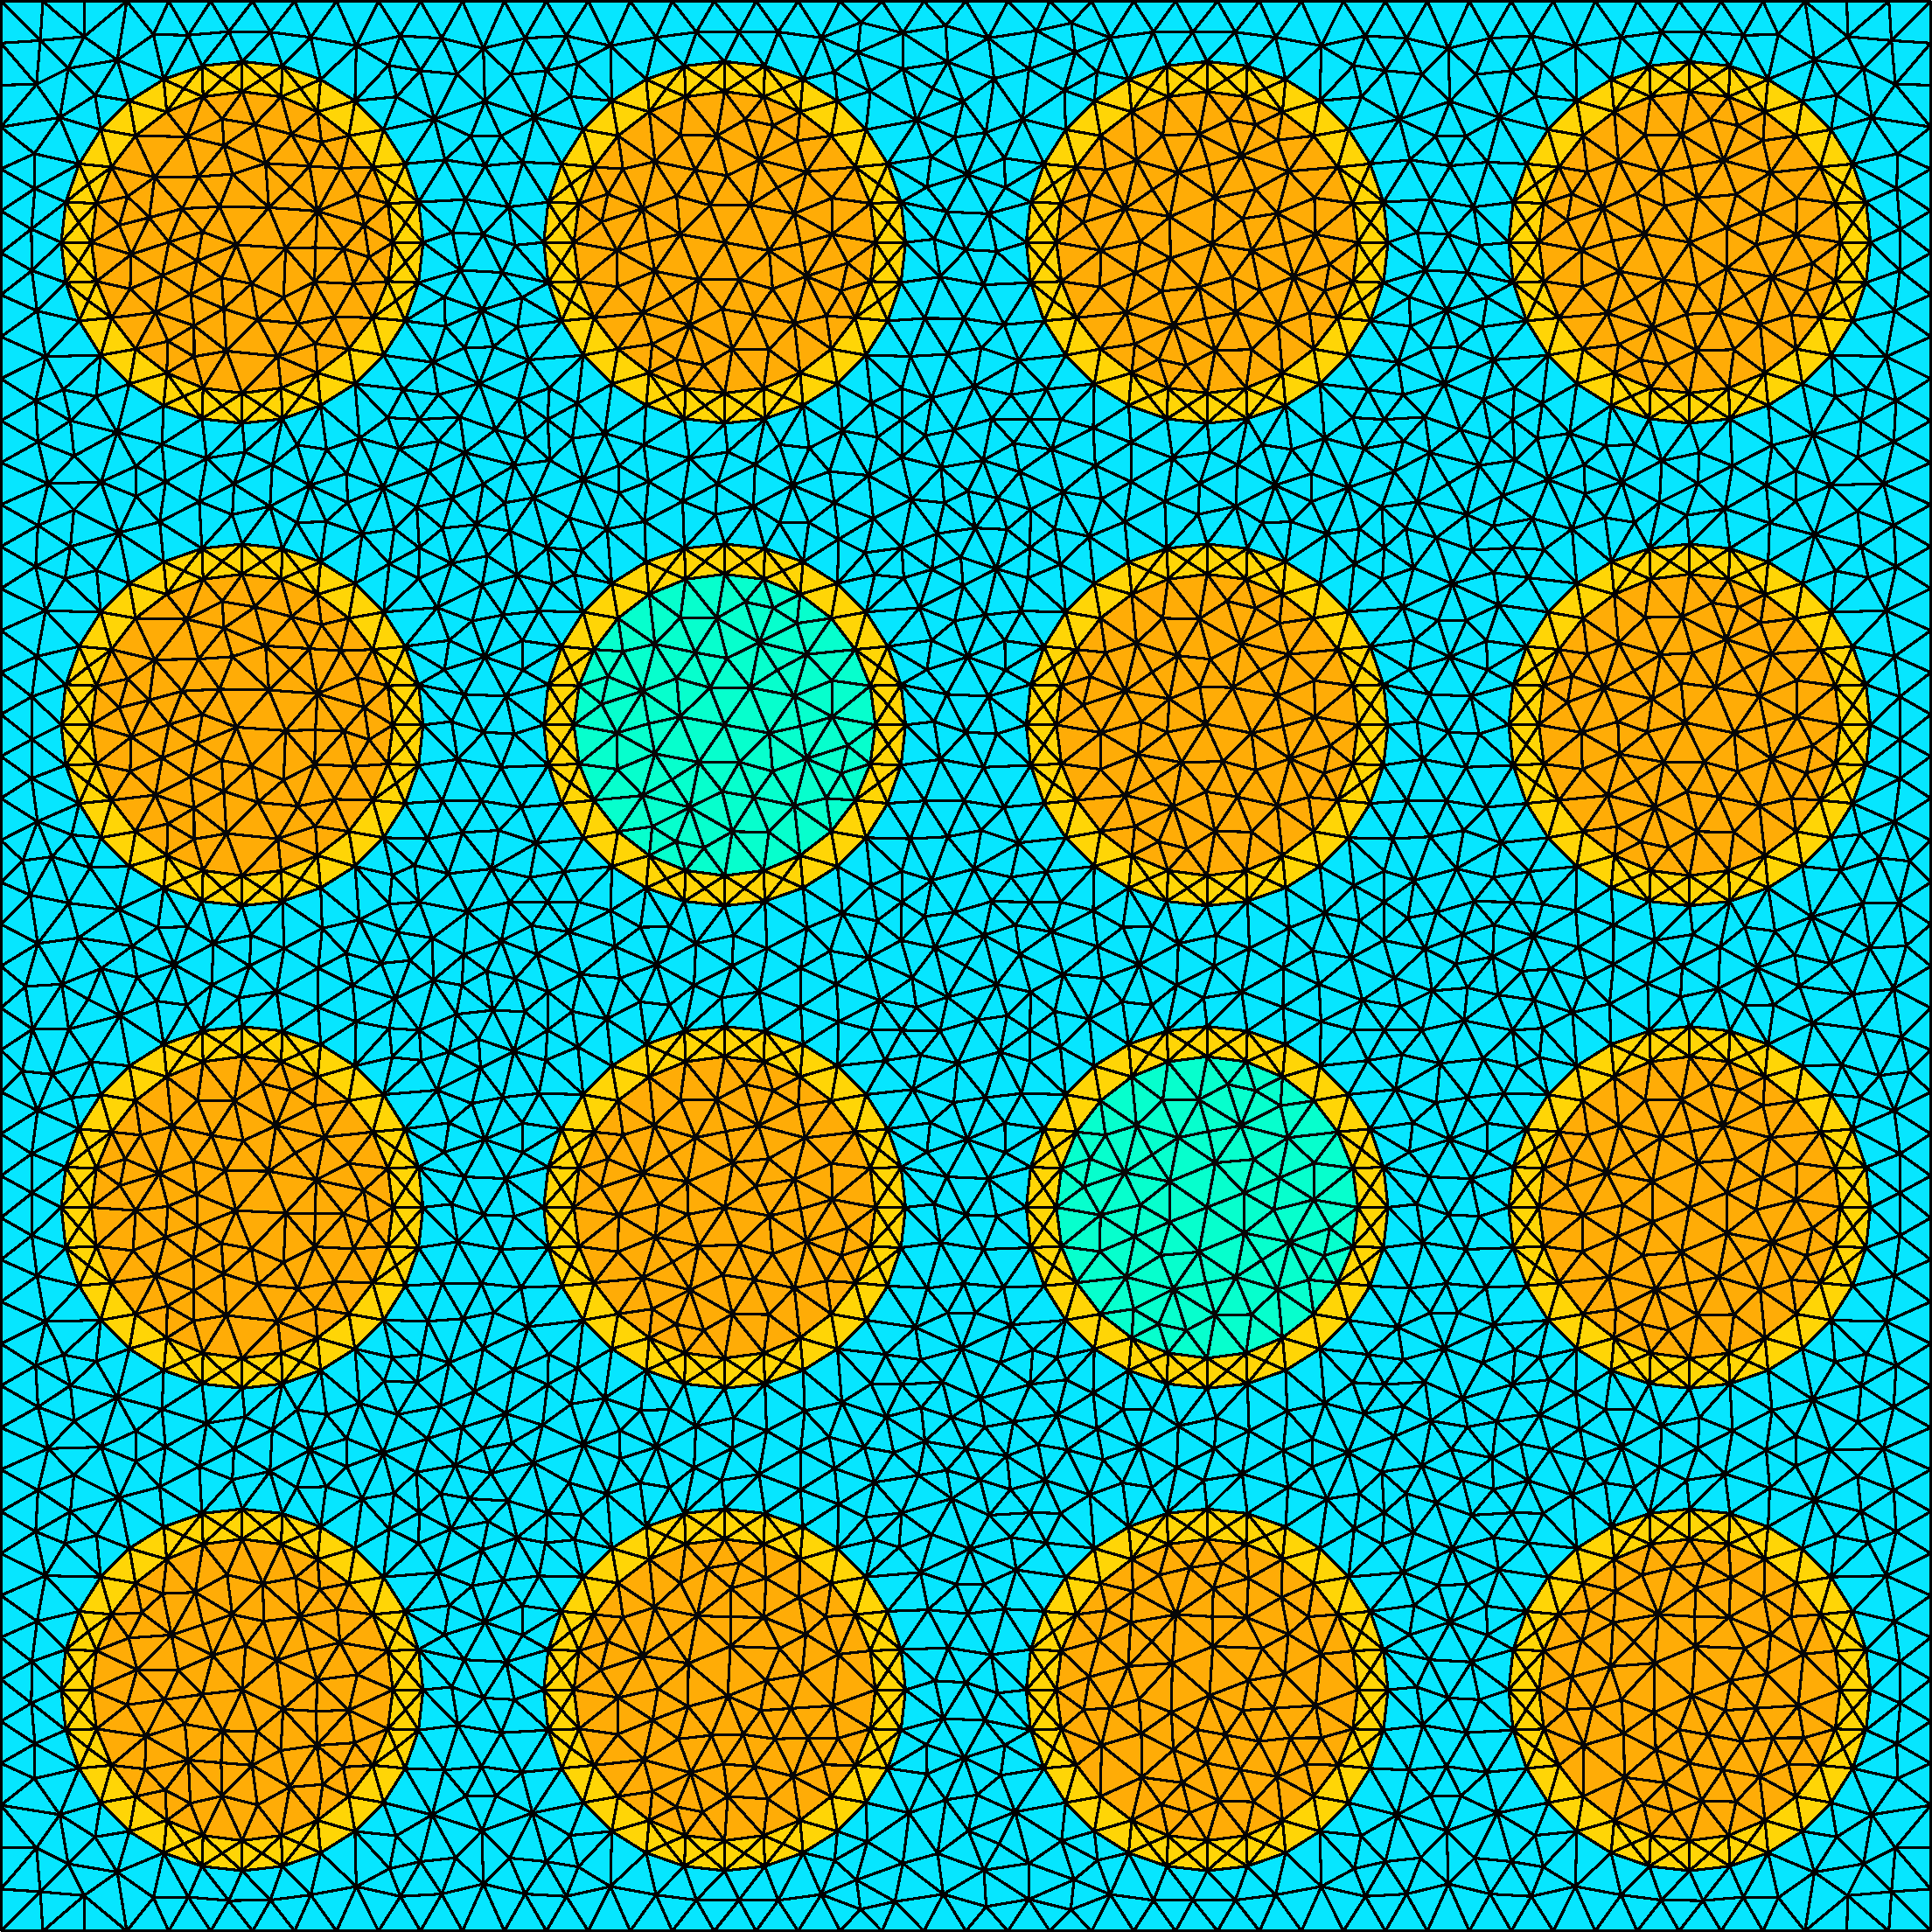
\includegraphics[width=0.6\linewidth]{graficos/bwr-gadolinio/bwr-gadolinio.pdf}
 \end{center}
\caption{\label{fig:bwr-mesh} Malla de celda BWR $\num{4} \times \num{4}$ obtenida a partir de gmsh~\cite{gmsh}. Los dos \emph{pins} que difieren de color son aquellos que poseen Gadolinio como veneno quemable. Aproximadamente, \num{6400} celdas forman la malla.}
\end{figure}

{
\begin{table}[h!]
\begin{center}
\begin{tabular}{lcccccc}
\small Material  & \small $g$ & \small $\Sigma^{f}_g$ & \small $\nu\Sigma^{f}_g$ & \small $\Sigma^{t}_g$ & \small $\Sigma^s_{g \rightarrow 1}$ & \small $\Sigma^s_{g \rightarrow 2}$ \\
\small Combustible & \tiny \num{1} & \tiny \num{7.22964e-3} & \tiny \num{1.86278e-2} & \tiny \num{3.62022e-1} & \tiny \num{3.33748e-1} & \tiny \num{6.64881e-4} \\
            & \tiny \num{2} & \tiny \num{1.41126e-1} & \tiny \num{3.44137e-1} & \tiny \num{5.72155e-1} & \tiny \num{0.0e-0}     & \tiny \num{3.80898e-1} \\
\small Zircaloy    & \tiny \num{1} & \tiny \num{0.0e-0} & \tiny \num{0.0e-0} & \tiny \num{2.74144e-1} & \tiny \num{2.72377e-1} & \tiny \num{1.90838e-4} \\
            & \tiny \num{2} & \tiny \num{0.0e-0} & \tiny \num{0.0e-0} & \tiny \num{2.80890e-1} & \tiny \num{0.0e-0}     & \tiny \num{2.77230e-1} \\
\small \emph{Pin} Gadolinio  & \tiny \num{1} & \tiny \num{6.97904e-3} & \tiny \num{1.79336e-2} & \tiny \num{3.71785e-1} & \tiny \num{3.38096E-1} & \tiny \num{6.92807e-4} \\
                      & \tiny \num{2} & \tiny \num{6.47524e-2} & \tiny \num{1.57929e-1} & \tiny \num{1.75e-0}    & \tiny \num{0.0e-0}     & \tiny \num{3.83204e-1} \\
\small Agua Liviana & \tiny \num{1} & \tiny \num{0.0e-0} & \tiny \num{0.0e-0} & \tiny \num{6.40711e-1} & \tiny \num{6.07382e-1} & \tiny \num{3.31316e-2} \\
             & \tiny \num{2} & \tiny \num{0.0e-0} & \tiny \num{0.0e-0} & \tiny \num{1.69131e-0} & \tiny \num{0.0e-0}     & \tiny \num{1.68428e-0} 
\end{tabular}
\caption{\label{tabla:xs-bwr} Secciones eficaces en~\si{\per\centi\metre} para el \emph{benchmark} de la celda BWR.}
\end{center}
\end{table}
}

\begin{figure}[!ht]
 \begin{center}
  \subfloat[\label{fig:bwr-flujo-rapido}]{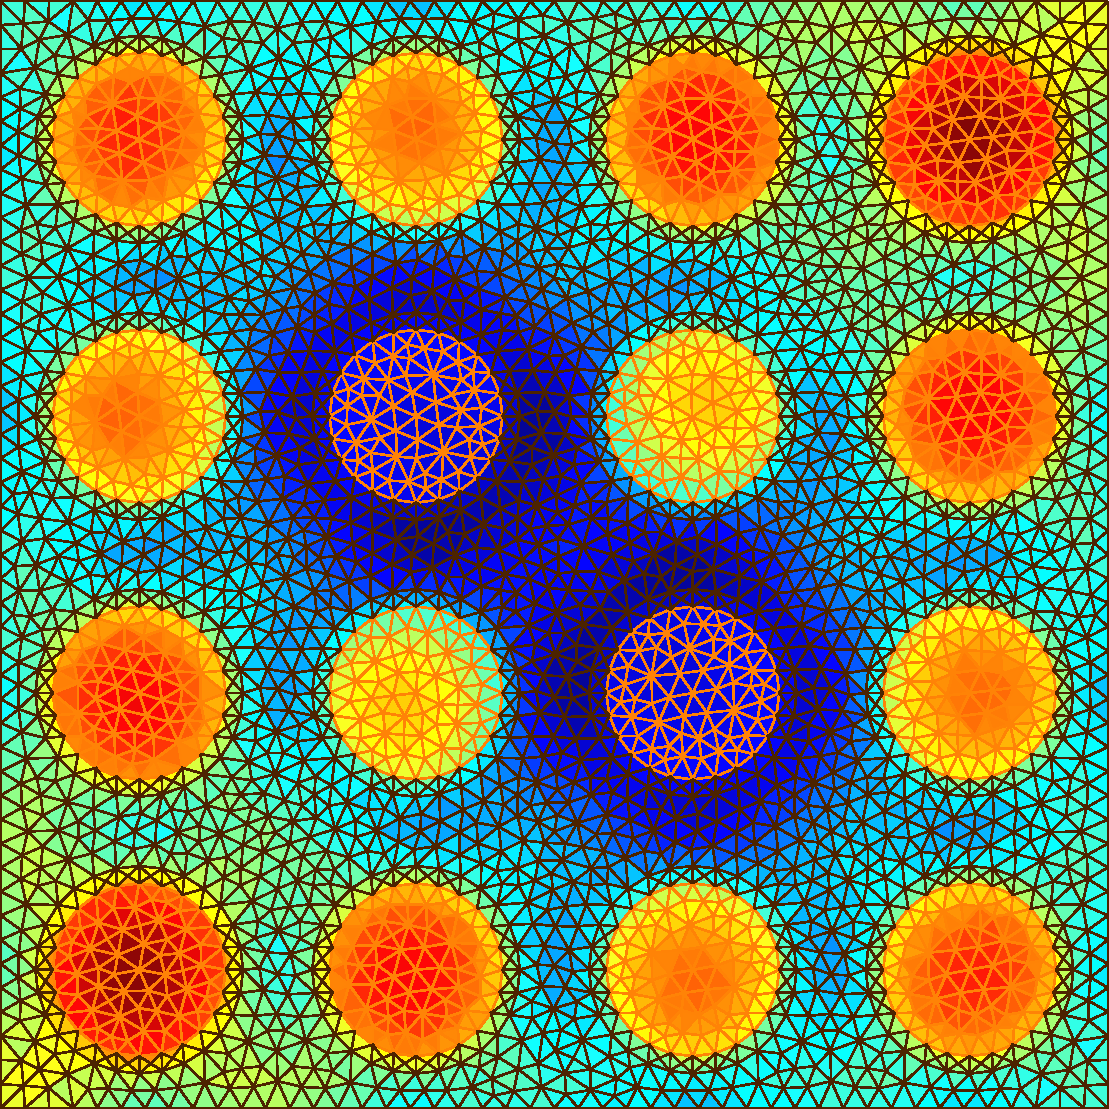
\includegraphics[width=0.485\linewidth]{graficos/flujos/gadolinio-rapido.pdf}}
  \subfloat[\label{fig:bwr-flujo-termico}]{ 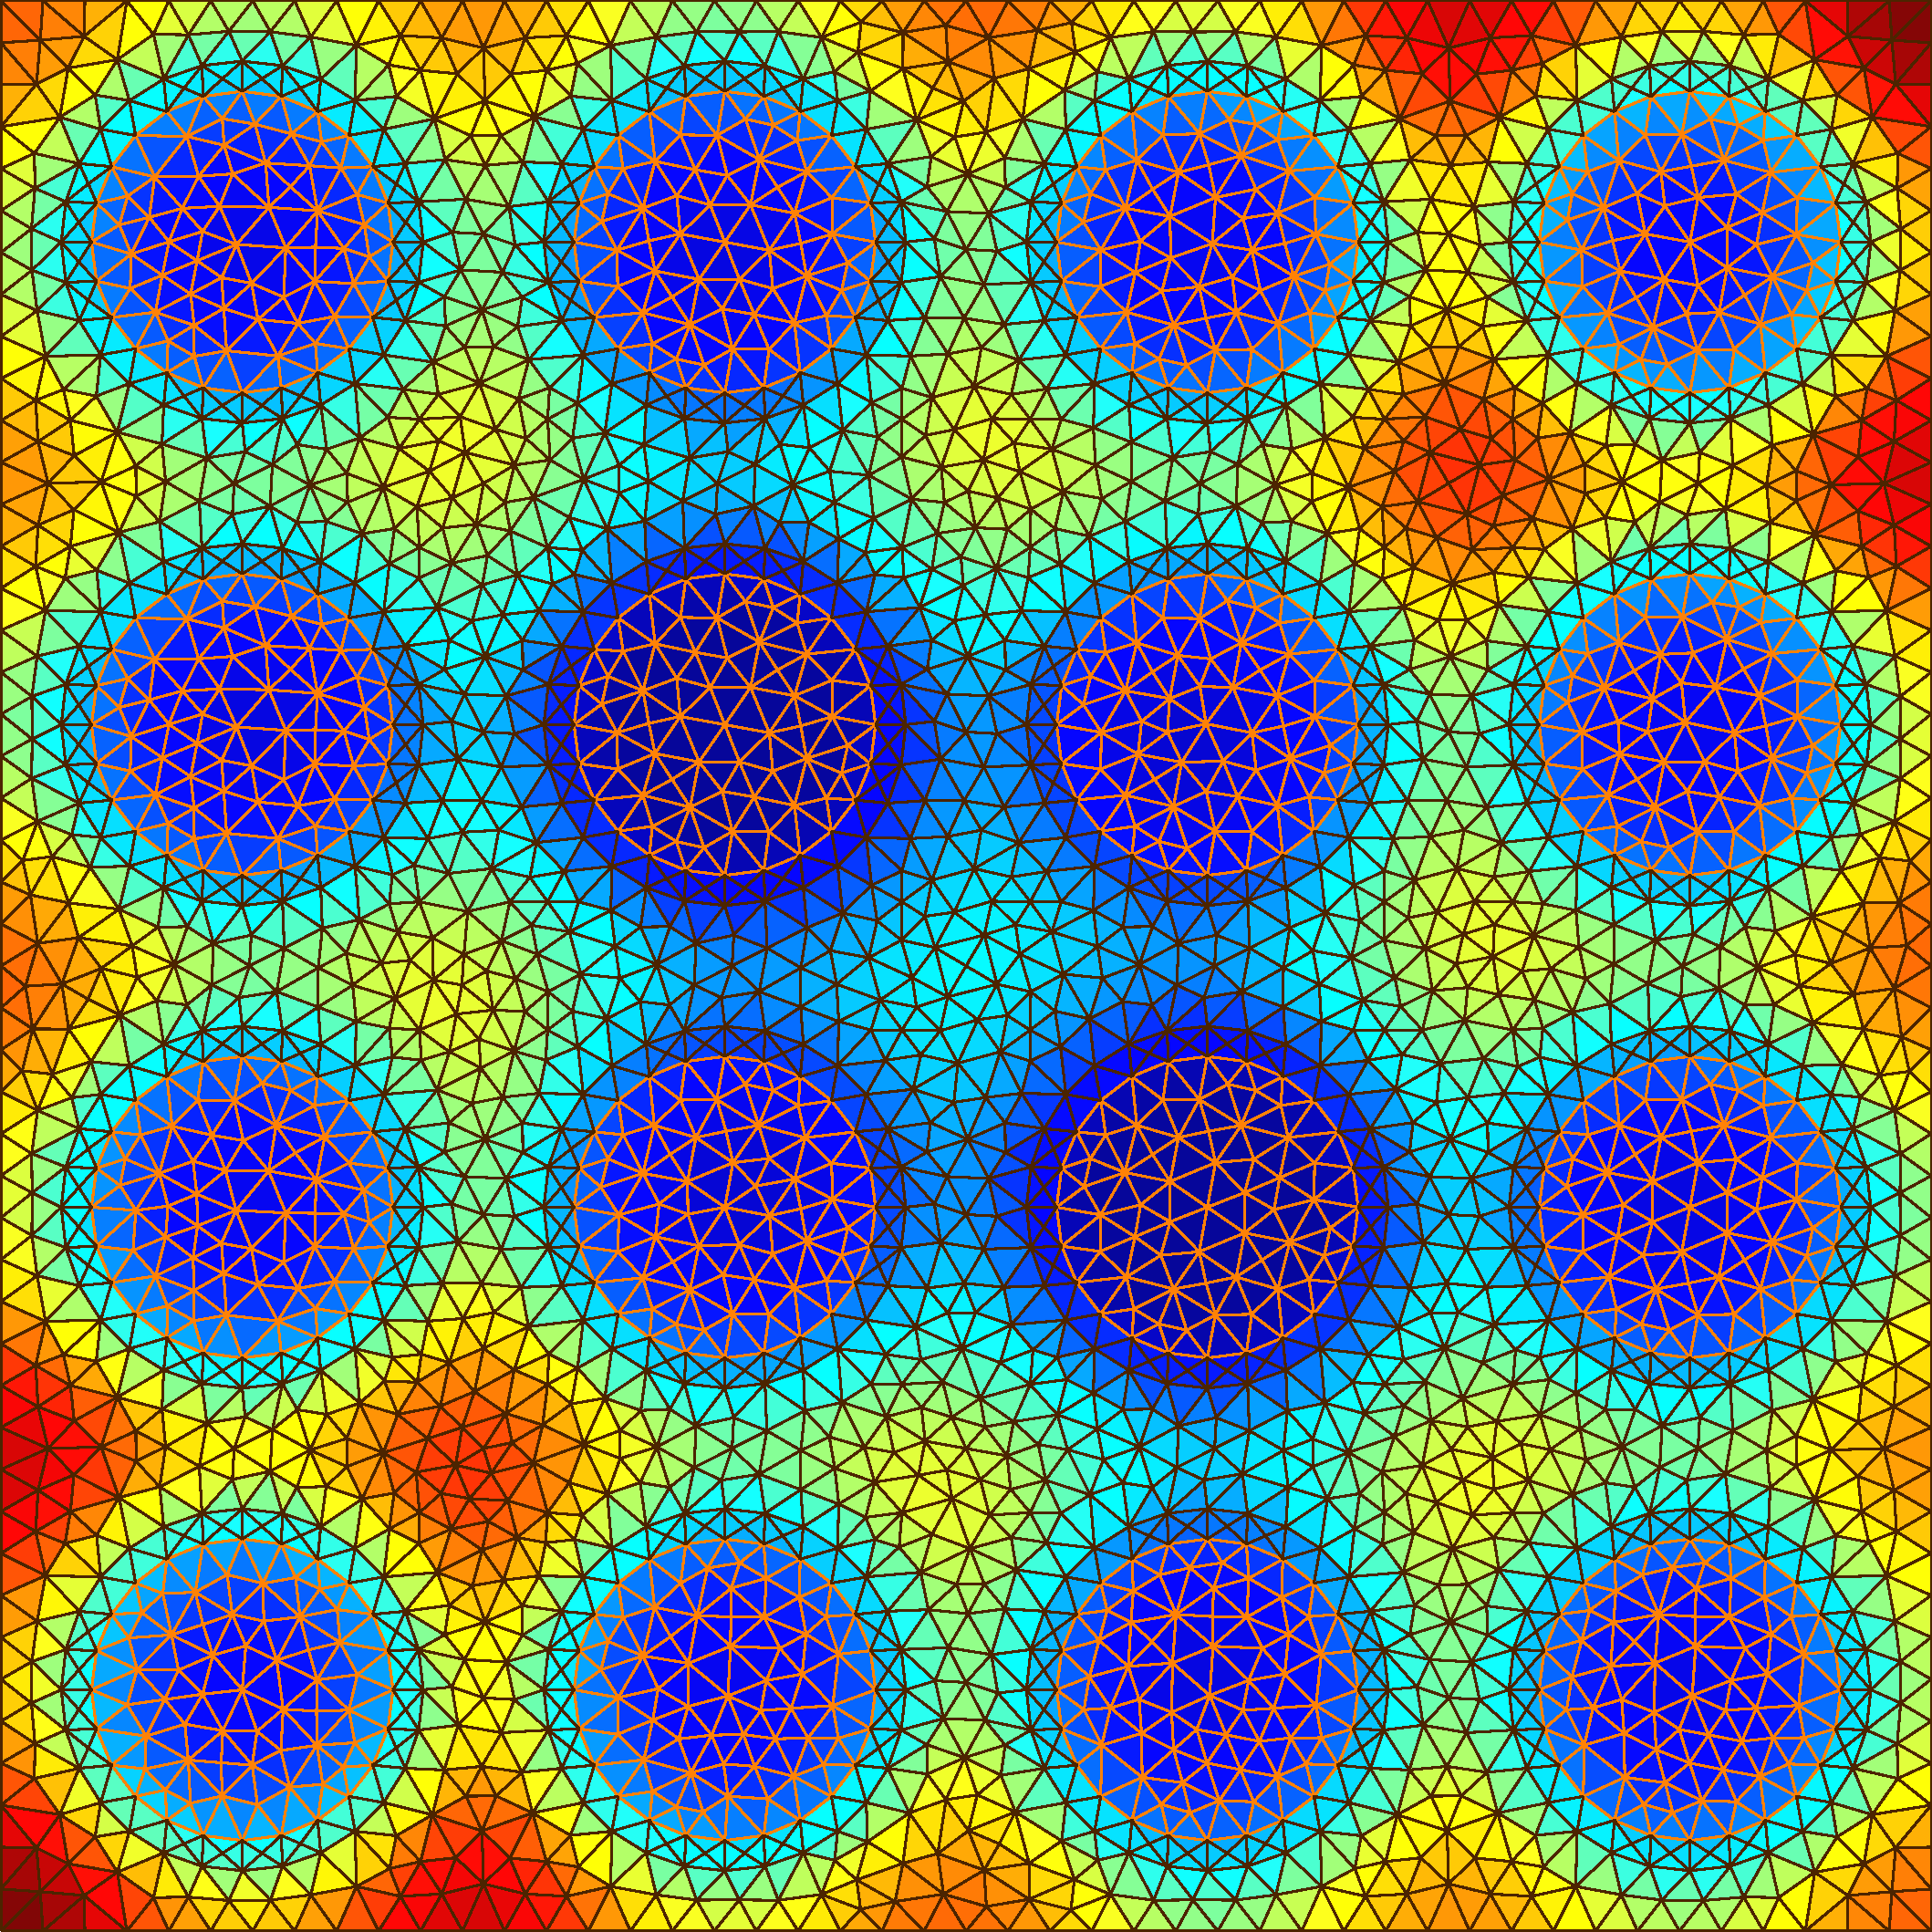
\includegraphics[width=0.485\linewidth]{graficos/flujos/gadolinio-termico.pdf}}\\
  \caption{Distribución espacial del flujo rápido~(\ref{fig:bwr-flujo-rapido}) y térmico~(\ref{fig:bwr-flujo-termico}) obtenido mediante la formulación moc en milonga.}
  \label{fig:bwr-flujos}
 \end{center}
\end{figure}



\section{Conclusiones}

mejorar la definicion de geometrias

\label{lastpage}


% \pagebreak
\printbibliography

\end{document}

